\documentclass{article}

\usepackage[utf8]{inputenc}
\usepackage[MeX]{polski}
\usepackage{lmodern}
\usepackage[T1]{fontenc}
\usepackage{indentfirst}
\usepackage[letterpaper,top=2cm,bottom=2cm,left=3cm,right=3cm,marginparwidth=1.75cm]{geometry}

% Useful packages
\usepackage{amsmath}
\usepackage{amssymb}
\usepackage{graphicx}
\usepackage[colorlinks=true, urlcolor=blue, linkcolor=black]{hyperref}
\usepackage{subcaption}
\usepackage{fancyhdr}
\usepackage{multicol}
\usepackage{float}
\pagestyle{fancy}
\fancyhf{} 
\fancyhead[L]{[MIOwAD] - raport MLP}
\fancyfoot[C]{\thepage}

\begin{document}

\title{
\large WYDZIAŁ MATEMATYKI I NAUK INFORMACYJNYCH \\
\large POLITECHNIKA WARSZAWSKA\\
\hrulefill \\
\LARGE MLP - Perceptrony Wielowarstwowe\\
\hrulefill \\
\large SPRAWOZDANIE}
\author{Kornel Tłaczała}

\maketitle
\tableofcontents
\newpage
\section*{NN1: Bazowa implementacja}
\addcontentsline{toc}{section}{NN1: Bazowa implementacja}
\subsection*{Cel}
\begin{enumerate}
    \item[a)] Stworzenie własnej, podstawowej implementacji sieci neuronowej, która będzie w stanie uczyć się na podstawie danych wejściowych i przewidywać wyniki zadania regresji. Zapewnienie możliwości łatwej zmiany architektury sieci oraz funkcji aktywacji.
    \item[b)] Ręczne dobranie parametrów sieci dla 3 architektur:
    \begin{itemize}
        \item 1 warstwa ukryta, 5 neuronów
        \item 1 warstwa ukryta, 10 neuronów
        \item 2 warstwy ukryte, 5 neuronów w każdej
    \end{itemize}
    oraz przetestowanie ich na 2 zbiorach danych:
    \begin{itemize}
        \item square-simple
        \item steps-large
    \end{itemize}
\end{enumerate}
\subsection*{Implementacja}

Model został zaimplementowany w Pythonie. W celu zapewnienia elastyczności oraz łatwości w rozwijaniu projektu implementacja została podzielona na klasy:
\begin{itemize}
    \item \textbf{\texttt{MLP()}} - klasa reprezentująca sieć neuronową, zawierająca metody do trenowania i przewidywania oraz wizualizacji wyników.
    \item \textbf{\texttt{Layer()}} - klasa reprezentująca pojedynczą warstwę sieci, zawierająca neurony oraz metody do obliczania aktywacji. Konieczne, ale i wygodne okazało się rozszerzenie tej klasy do klas \textbf{\texttt{FirstLayer}} i \textbf{\texttt{LastLayer}}, które reprezentują odpowiednio warstwę wejściową i wyjściową i miały częstą inną funckję aktywacji, bądź sposób aktualizacji wag. To właśnie każda warstwa przechowywała informację o wartościach wag, biasów oraz informację o wykorzystywanej funkcji aktywacji.
    \item \textbf{\texttt{MLPArchitecture()}} - klasa reprezentująca architekturę \texttt{MLP}, zapewniająca możliwość łatwego tworzenia różnych konfiguracji sieci neuronowych poprzez definiowanie liczby warstw i neuronów w każdej z nich
    \item \textbf{\texttt{Dataset()}} - klasa reprezentująca zbiór danych, zawierająca metody do ładowania danych z plików CSV oraz dzielenia ich na zbiory treningowe i testowe. Automatyzuje ona normalizację danych. Wspomaga klasę \texttt{MLP} w reprezentacji zbioru danych. Jej metody przyjmując przewidywania sieci, zwracają odpowiednie metryki jakości predykcji, w tym liczą funkcję straty.
\end{itemize}

\subsection*{Zbiory danych}
\begin{figure}[H]
    \centering
    \begin{subfigure}[b]{0.45\textwidth}
        \centering
        \includegraphics[width=\textwidth]{img/nn1/steps-large.png}
        \label{fig:steps-large}
    \end{subfigure}
    \hfill
    \begin{subfigure}[b]{0.45\textwidth}
        \centering
        \includegraphics[width=\textwidth]{img/nn1/square-simple.png}
        \label{fig:square-simple}
    \end{subfigure}
    \caption{Prezentacja zbiorów steps-large i square-simple}
\end{figure}

\subsection*{Wyniki - steps-large}
\begin{table}[H]
    \centering
    \begin{tabular}{|c|c|c|}
        \hline
        Architektura & MSE (train) & MSE (test) \\
        \hline
        1-5-1 & 0.02 & 0.00 \\
        1-10-1 & 0.02 & 0.00 \\
        1-5-5-1 & 0.00 & 0.00 \\
        \hline
    \end{tabular}
    \caption{Wartości funkcji straty (MSE) dla zbioru steps-large}
\end{table}
\begin{figure}[H]
    \centering
    \begin{subfigure}[b]{0.45\textwidth}
        \centering
        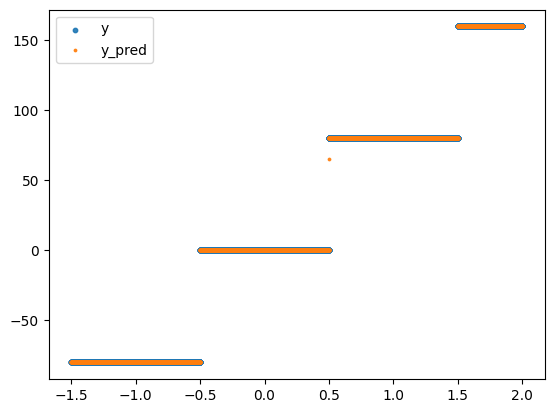
\includegraphics[width=\textwidth]{img/nn1/steps-large_train_1-5-1.png}
        \caption{1-5-1: MSE = 0.02 (train)}
    \end{subfigure}
    \hfill
    \begin{subfigure}[b]{0.45\textwidth}
        \centering
        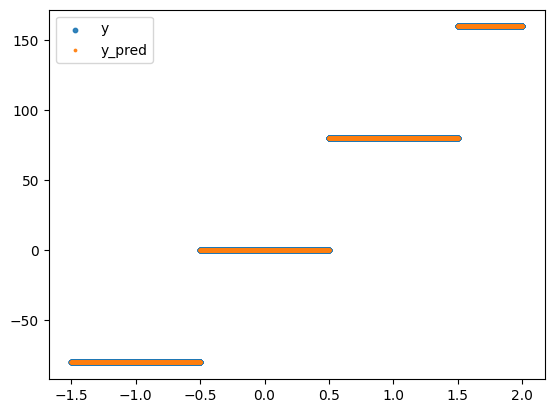
\includegraphics[width=\textwidth]{img/nn1/steps-large_train_1-5-5-1.png}
        \caption{1-5-5-1: MSE = 0.00 (train)}
    \end{subfigure}
    \caption{Porównanie wyników dla architektur 1-5-1 i 1-5-5-1 na zbiorze steps-large}
\end{figure}
\subsection*{Wyniki - square-simple}
Dla zbioru square-simple najsensowniejsze dopasowanie udało się uzyskać dla architektury 1-5-5-1. Dla tej architektury MSE wynosiło mniej niż 1 zarówno na zbiorze treningowym, jak i testowym. 
\begin{table}[H]
    \centering
    \begin{tabular}{|c|c|c|}
        \hline
        & MSE (train) & MSE (test) \\
        \hline
        Wynik & 0.74 & 0.78 \\
        \hline
    \end{tabular}
    \caption{Wartości funkcji straty (MSE) dla zbioru square-simple}
\end{table}
\begin{figure}[H]
    \centering
    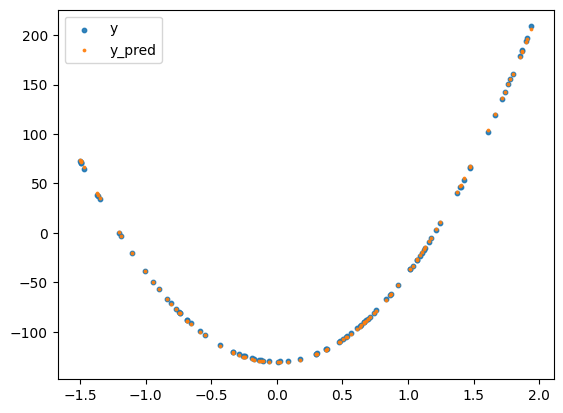
\includegraphics[width=0.6\textwidth]{img/nn1/square-simple_train_1-5-5-1.png}
    \caption{1-5-5-1: MSE = 0.74 (train)}
\end{figure}

\section*{NN2: Propagacja wsteczna}
\addcontentsline{toc}{section}{NN2: Propagacja wsteczna}
\subsection*{Cel}
\begin{enumerate}
    \item[a)] Zaimplementowanie algorytmu propagacji wstecznej (backpropagation) w celu automatycznego wyznaczania gradientów i aktualizacji wag w sieci neuronowej.
    \item[b)] Przeprowadzenie eksperymentów porównujących skuteczność uczenia sieci z propagacją wsteczną na zbiorach danych:
    \begin{itemize}
        \item square-simple
        \item steps-small
        \item multimodal-large
    \end{itemize}
    \item[c)] Analiza wpływu liczby epok, współczynnika uczenia oraz architektury sieci na proces uczenia i jakość predykcji.
\end{enumerate}

\subsection*{Implementacja}
Na tym etapie do implementacji zostały dodane następujące funkcjonalności:
\begin{itemize}
    \item klasa \textbf{\texttt{Initializer()}} - jej podklasy odpowiadają za inicjalizację wag i biasów w sieci neuronowej. Wykorzystano różne metody inicjalizacji, takie jak \textit{Xavier} i \textit{He}, które są dostosowane do różnych funkcji aktywacji.
    \item klasa \textbf{\texttt{ActivationFunction()}} - jej podklasy implementują różne funkcje aktywacji, takie jak \textit{ReLU}, \textit{sigmoid} i \textit{tanh}. Każda z tych funkcji jest dostosowana do specyfiki danych wejściowych oraz architektury sieci.
    \item klasa \textbf{\texttt{ModelHistory()}} - odpowiada za przechowywanie i analizę historii uczenia, w tym wartości funkcji straty (MSE) dla zbiorów treningowych i testowych. Umożliwia zapamiętanie parametrów sieci neuronowej oraz wygenerowanie wykresów ilustrujących historię procesu uczenia.
    \item \textbf{Mechanizm backpropagacji} - podzielony na trzy etapy: \texttt{forward} (w celu wyliczenia aktualnej predykcji), \texttt{backward} (w celu wyliczenia błędów oraz zmian gradientów) oraz \texttt{update} (aktualizacja wag i biasów w sieci neuronowej). Zapewniona została możliwość trenowania modelu z wykorzystaniem \texttt{SGD}, \texttt{mini-batch} oraz \texttt{batch} (uczenia na całym zbiorze danych). Zauważalne było, że model pracuje szybciej (pod względem mijających epok) przy użyciu mniejszych partii danych, (\texttt{mini-batch}, lub w szczególności \texttt{SGD}). Wiązało się to jednak z mniejszą stabilnością wyników.
\end{itemize}

\subsection*{Zbiory danych}
\begin{figure}[H]
    \centering
    \begin{subfigure}[b]{0.3\textwidth}
        \centering
        \includegraphics[width=\textwidth]{img/nn2/square-simple.png}
        \caption{square-simple}
    \end{subfigure}
    \hfill
    \begin{subfigure}[b]{0.3\textwidth}
        \centering
        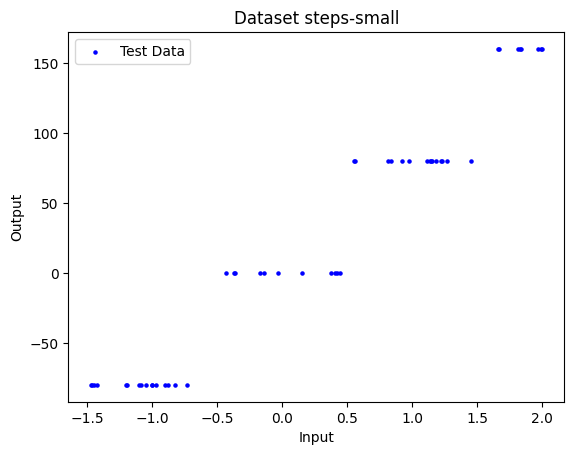
\includegraphics[width=\textwidth]{img/nn2/steps-small.png}
        \caption{steps-small}
    \end{subfigure}
    \hfill
    \begin{subfigure}[b]{0.3\textwidth}
        \centering
        \includegraphics[width=\textwidth]{img/nn2/multimodal-large.png}
        \caption{multimodal-large}
    \end{subfigure}
    \caption{Prezentacja zbiorów danych: square-simple, steps-small, multimodal-large}
\end{figure}
\subsection*{Trening}
Dla każdego ze zbiorów został wytrenowany model. Trening odbywał się zarówno na całym zbiorze danych w każdej iteracji, jak i przy użyciu mini-batch oraz SGD. W przypadku zbioru multimodal-large, ze względu na jego dużą wielkość, lepsze rezultaty zdawał się osiągać trening z użyciem mini-batch. Dane treningowe w zbiorze steps-large okazały się przesunięte w stosunku do danych testowych, co w połączeniu ze skokową naturą danych, skutkowało dużymi wartościami funkcji straty (MSE) dla tego zbioru w przypadku ewaluacji na zbiorze treningowym.
\subsection*{Square-simple}
\subsubsection*{Wykorzystano architekturę 1-50-100-50-1}
\begin{figure}[H]
    \centering
    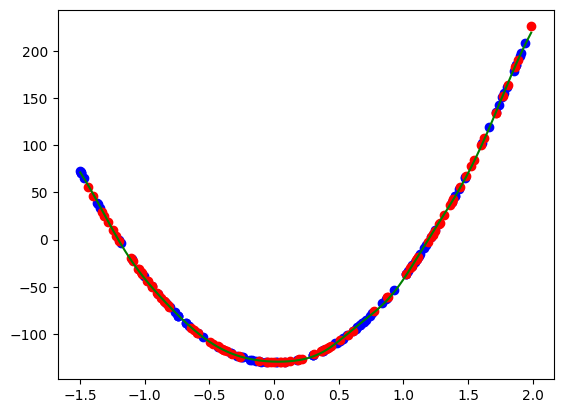
\includegraphics[width=0.8\textwidth]{img/nn2/square-simple_batch_training_fit.png}
    \caption{Dopasowanie modelu do zbioru square-simple przy użyciu batch}
\end{figure}

\subsubsection*{Wyniki}
\begin{table}[H]
    \centering
    \begin{tabular}{|c|c|c|c|}
        \hline
        Metoda & Liczba epok & MSE (train) & MSE (test) \\
        \hline
        batch & 9000 & 1.51 & 1.98 \\
        mini-batch & 3000 & 0.70 & 1.05 \\
        \hline
    \end{tabular}
    \caption{Model na mini-batch uczył się krócej, ale osiągnął lepsze wyniki.}
\end{table}

\subsubsection*{Historia uczenia (loss curves)}
Poniższe wykresy przedstawiają porównanie procesu nauki modelu przy użyciu metod batch oraz mini-batch. Można zauważyć, że model przy uczeniu mini-batch działał bardziej chaotycznie, ale szybciej osiągał lepsze rezultaty. W przypadku batch model uczył się wolniej, ale stabilniej.
\begin{figure}[H]
    \centering
    \begin{subfigure}[b]{0.48\textwidth}
        \centering
        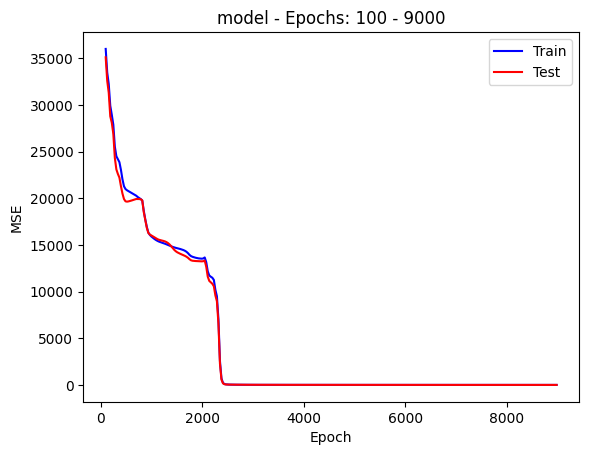
\includegraphics[width=\textwidth]{img/nn2/square-simple_batch_training_history.png}
        \caption{Przebieg funkcji straty (MSE) podczas uczenia na zbiorze square-simple (batch)}
    \end{subfigure}
    \hfill
    \begin{subfigure}[b]{0.48\textwidth}
        \centering
        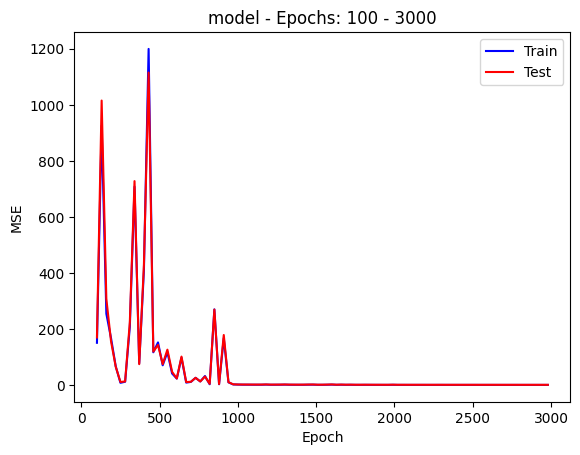
\includegraphics[width=\textwidth]{img/nn2/square-simple_mini-batch_training_history.png}
        \caption{Przebieg funkcji straty (MSE) podczas uczenia na zbiorze square-simple (mini-batch)}
    \end{subfigure}
    \caption{Porównanie procesu uczenia (batch vs mini-batch) na zbiorze square-simple}
\end{figure}

\subsection*{Steps-small}
\subsubsection*{Wykorzystano architekturę 1-50-100-50-1}
\begin{figure}[H]
    \centering
    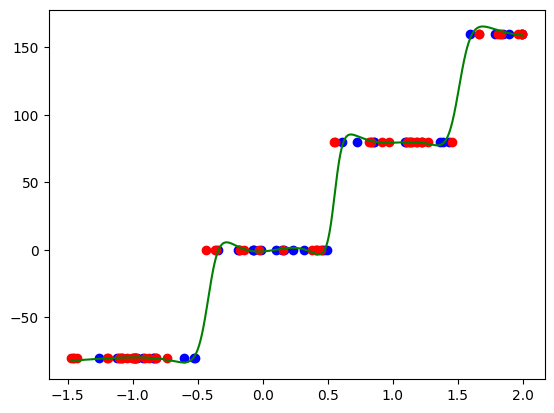
\includegraphics[width=0.8\textwidth]{img/nn2/steps-small_mini-batch_training_fit.png}
    \caption{Dopasowanie modelu do zbioru steps-small przy użyciu mini-batch}
\end{figure}

\subsubsection*{Wyniki}
\begin{table}[H]
    \centering
    \begin{tabular}{|c|c|c|c|}
        \hline
        Metoda & Liczba epok & MSE (train) & MSE (test) \\
        \hline
        batch & 103000 & 2.66 & 109.46 \\
        mini-batch & 17000 & 3.98 & 104.91 \\
        \hline
    \end{tabular}
    \caption{Porównanie wyników dla batch i mini-batch na zbiorze steps-small.}
\end{table}

\subsection*{Multimodal-large}
\subsubsection*{Wykorzystano architekturę 1-50-100-50-1}
\begin{figure}[H]
    \centering
    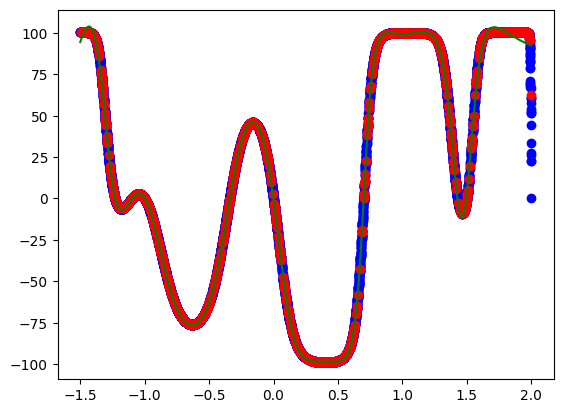
\includegraphics[width=0.8\textwidth]{img/nn2/multimodal-large_mini-batch_training_fit.png}
    \caption{Dopasowanie modelu do zbioru multimodal-large przy użyciu mini-batch}
\end{figure}

\subsubsection*{Wyniki}
\begin{table}[H]
    \centering
    \begin{tabular}{|c|c|c|c|}
        \hline
        Metoda & Liczba epok & MSE (train) & MSE (test) \\
        \hline
        mini-batch & 700 & 7.47 & 3.78 \\
        \hline
    \end{tabular}
    \caption{Porównanie wyników dla mini-batch na zbiorze multimodal-large.}
\end{table}

% \section*{NN3: Implementacja momentu i normalizacji gradientu (RMSProp)}
\section*{NN3: Implementacja momentu i normalizacji (RMSProp)}
\addcontentsline{toc}{section}{NN3: Implementacja momentu i normalizacji gradientu (RMSProp)}
\subsection*{Cel}
\begin{enumerate}
    \item[a)] Dodanie do implementacji sieci neuronowej mechanizmu uczenia z momentem oraz normalizacji gradientu RMSProp w celu poprawy procesu uczenia na trudnych zbiorach danych.
    \item[b)] Przeprowadzenie eksperymentów porównujących skuteczność uczenia z momentem i RMSProp względem klasycznego SGD lub mini-batch na zbiorach danych:
    \begin{itemize}
        \item square-large
        \item steps-large
        \item multimodal-large
    \end{itemize}
    \item[c)] Analiza wpływu parametrów momentu i RMSProp (np. współczynnika momentu, parametru $\beta$) na szybkość i stabilność uczenia.
\end{enumerate}

\subsection*{Implementacja}
Do metody \texttt{train}() dodany został parametr \texttt{optimizer}, który pozwala na wybór metody optymalizacji. Dodatkowo można również podać parametry specyficzne dla danej metody, takie jak współczynnik momentu \texttt{momentum\_lambda} dla metody z momentem oraz \texttt{rms\_beta} dla RMSProp.

\subsection*{Zbiory danych}
\begin{figure}[H]
    \centering
    \begin{subfigure}[b]{0.3\textwidth}
        \centering
        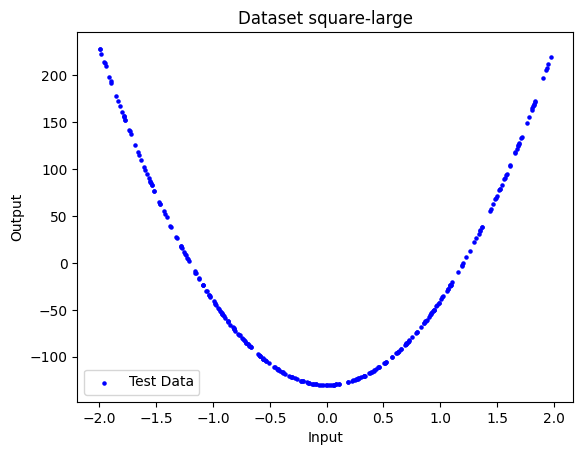
\includegraphics[width=\textwidth]{img/nn3/square-large.png}
        \caption{square-large}
    \end{subfigure}
    \hfill
    \begin{subfigure}[b]{0.3\textwidth}
        \centering
        \includegraphics[width=\textwidth]{img/nn3/steps-large.png}
        \caption{steps-large}
    \end{subfigure}
    \hfill
    \begin{subfigure}[b]{0.3\textwidth}
        \centering
        \includegraphics[width=\textwidth]{img/nn3/multimodal-large.png}
        \caption{multimodal-large}
    \end{subfigure}
    \caption{Prezentacja zbiorów danych: square-large, steps-large, multimodal-large}
\end{figure}

\subsection*{Square-large}

\begin{figure}[H]
    \centering
    \begin{subfigure}[b]{0.48\textwidth}
        \centering
        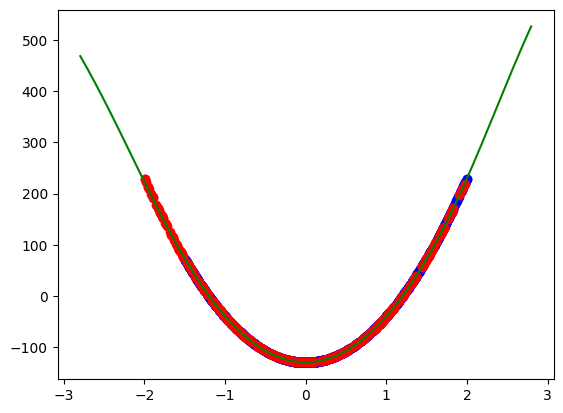
\includegraphics[width=\textwidth]{img/nn3/square-large_momentum_fit.png}
        \caption{Momentum: predykcja na zielono}
    \end{subfigure}
    \hfill
    \begin{subfigure}[b]{0.48\textwidth}
        \centering
        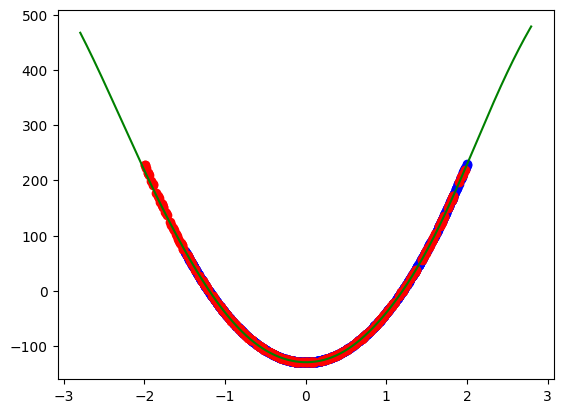
\includegraphics[width=\textwidth]{img/nn3/square-large_rms_fit.png}
        \caption{RMSProp: predykcja na zielono}
    \end{subfigure}
    \caption{Porównanie dopasowania na zbiorze square-large}
\end{figure}

\subsubsection*{Wyniki}
\begin{table}[H]
    \centering
    \begin{tabular}{|c|c|c|c|}
        \hline
        Metoda optymalizacji & Liczba epok & MSE (train) & MSE (test) \\
        \hline
        Momentum & 3778 & 0.27 & 1.05 \\
        RMSProp & 129 & 0.56 & 3.54 \\
        \hline
    \end{tabular}
    \caption{Porównanie skuteczności optymalizatorów Momentum i RMSProp na zbiorze square-large (MSE dla zbioru treningowego i testowego).}
\end{table}

\subsubsection*{Obserwacje}
Trening z wykorzystaniem momentu przebiegał w sposób jednostajny. Modelowi udało się "dociągnąć" odstające (przez brak danych treningowych) ramię, co pozwoliło na osiągnięcie satysfakcjonujących wyników na zbiorze testowym. W przypadku RMSProp model uczył się znacznie szybciej, (tylko 129 epok!) i osiągnął podobne wyniki, chociaż dla tego zbioru moment wydaje się być lepszym rozwiązaniem. 

\subsection*{Steps-large}

Dla tego zbioru danych, przy treningu z momentem, najlepiej zdawało się funkcjonować SGD. Z kolei RMSProp najlepiej działał przy użyciu mini-batch.

\begin{figure}[H]
    \centering
    \begin{subfigure}[b]{0.48\textwidth}
        \centering
        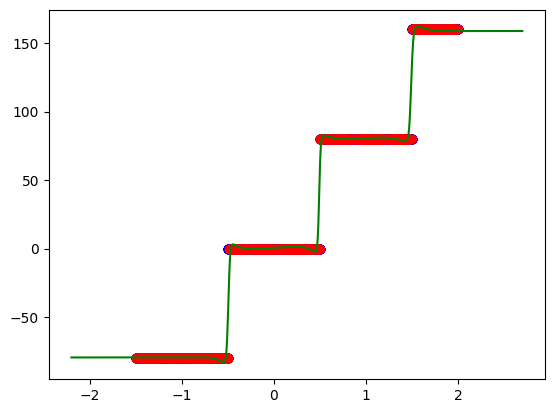
\includegraphics[width=\textwidth]{img/nn3/steps-large_momentum_fit.png}
        \caption{Momentum: predykcja na zielono}
    \end{subfigure}
    \hfill
    \begin{subfigure}[b]{0.48\textwidth}
        \centering
        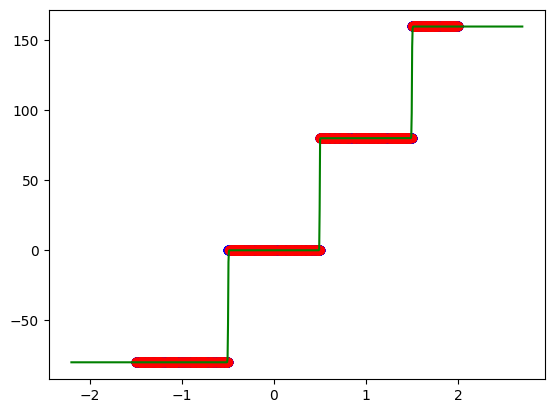
\includegraphics[width=\textwidth]{img/nn3/steps-large_rms_fit.png}
        \caption{RMSProp: predykcja na zielono}
    \end{subfigure}
    \caption{Porównanie dopasowania na zbiorze steps-large}
\end{figure}

\subsubsection*{Wyniki}
\begin{table}[H]
    \centering
    \begin{tabular}{|c|c|c|c|}
        \hline
        Metoda optymalizacji & Liczba epok & MSE (train) & MSE (test) \\
        \hline
        Momentum & 180 & 25.71 & 15.27 \\
        RMSProp & 2139 & 5.88 & 0.7 \\
        \hline
    \end{tabular}
    \caption{Porównanie skuteczności optymalizatorów Momentum i RMSProp na zbiorze steps-large (MSE dla zbioru treningowego i testowego).}
\end{table}

\subsubsection*{Obserwacje}
W wypadku tego zbioru danych, RMSProp okazał się znacznie lepszym rozwiązaniem niż Momentum. Model z wykorzystaniem RMSProp osiągnął bardzo dobre wyniki na zbiorze testowym, podczas gdy model z momentem po osiągnięciu MSE ok. 15, zaczął się przeuczać a wartość na zbiorze testowym wzrastała.

\subsection*{Multimodal-large}

\begin{figure}[H]
    \centering
    \begin{subfigure}[b]{0.48\textwidth}
        \centering
        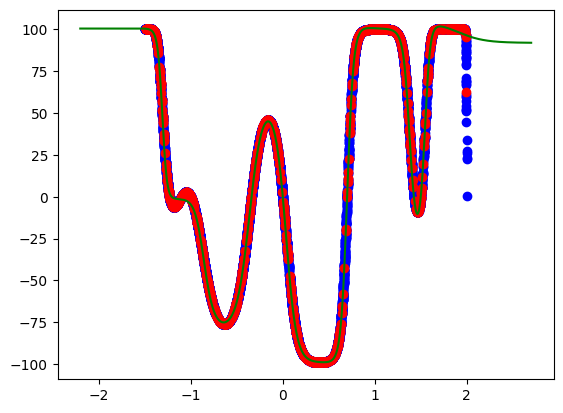
\includegraphics[width=\textwidth]{img/nn3/multimodal-large_momentum_fit.png}
        \caption{Momentum: predykcja na zielono}
    \end{subfigure}
    \hfill
    \begin{subfigure}[b]{0.48\textwidth}
        \centering
        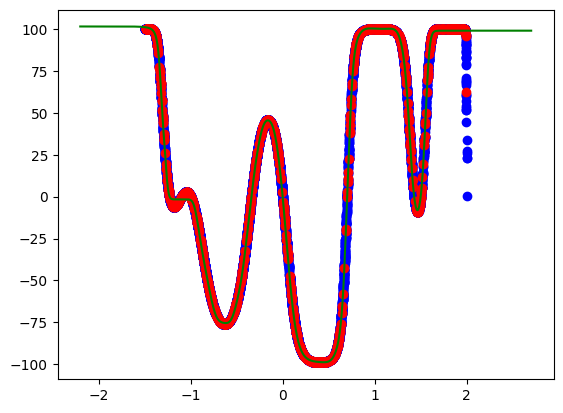
\includegraphics[width=\textwidth]{img/nn3/multimodal-large_rms_fit.png}
        \caption{RMSProp: predykcja na zielono}
    \end{subfigure}
    \caption{Porównanie dopasowania na zbiorze multimodal-large}
\end{figure}

\subsubsection*{Wyniki}
\begin{table}[H]
    \centering
    \begin{tabular}{|c|c|c|c|}
        \hline
        Metoda optymalizacji & Liczba epok & MSE (train) & MSE (test) \\
        \hline
        Momentum & 134 & 7.9 & 3.17 \\
        RMSProp & 1194 & 7.34 & 2.21 \\
        \hline
    \end{tabular}
    \caption{Porównanie skuteczności optymalizatorów Momentum i RMSProp na zbiorze multimodal-large (MSE dla zbioru treningowego i testowego).}
\end{table}

\subsubsection*{Obserwacje}
Na tym zbiorze oba modele poradziły sobie bardzo dobrze.

\subsection*{Ogólne spostrzeżenia}
Niezależnie od modelu korzystne było stopniowe zmniejszanie learning-rate w trakcie uczenia. W przypadku uczenia z momentem, lambda w zakresie 0.7-0.9 dawała najlepsze rezultaty. Ważne było jednak stopniowe zwiększanie tego parametru, od wartości 0.3 przez 0.5 do 0.7. Pozwalało to uniknąć natychmiastowego wybicia wag w nieoczekiwanym kierunku.


\section*{NN4: Klasyfikacja - implementacja z softmax}
\addcontentsline{toc}{section}{NN4: Klasyfikacja - implementacja z softmax}
\subsection*{Cel}
\begin{enumerate}
    \item[a)] Rozszerzenie implementacji sieci neuronowej o możliwość rozwiązywania zadań klasyfikacyjnych poprzez dodanie funkcji aktywacji softmax.
    \item[b)] Implementacja funkcji kosztu cross-entropy odpowiedniej dla klasyfikacji wieloklasowej.
    \item[c)] Przetestowanie działania sieci na wybranych zbiorach danych klasyfikacyjnych oraz analiza jakości predykcji.
\end{enumerate}

\subsection*{Implementacja}
Na tym etapie zaimplementowana została funkcja aktywacji \texttt{softmax} jako podklasa klasy \texttt{ActivationFunction()}, która jest wykorzystywana w warstwie wyjściowej sieci neuronowej do przekształcania wyników na prawdopodobieństwa dla poszczególnych klas. Dodatkowo, wprowadzono funkcję kosztu \texttt{cross-entropy}, która jest odpowiednia dla zadań klasyfikacyjnych i pozwala na efektywne uczenie się modelu.
\newpage

\subsection*{Zbiory danych}
\begin{figure}[H]
    \centering
    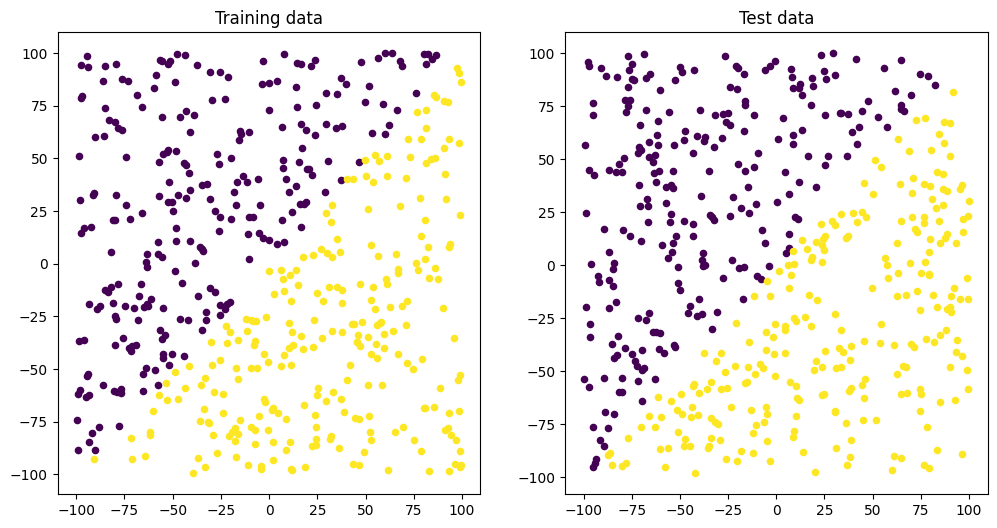
\includegraphics[width=0.7\textwidth]{img/nn4/easy.png}
    \caption{Dataset: easy}
\end{figure}
\begin{figure}[H]
    \centering
    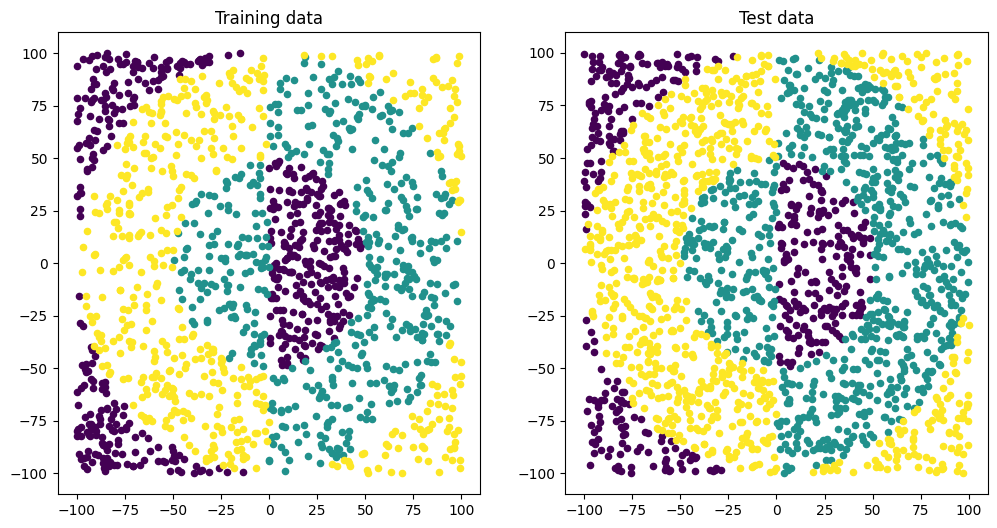
\includegraphics[width=0.7\textwidth]{img/nn4/rings3.png}
    \caption{Dataset: rings3}
\end{figure}
\begin{figure}[H]
    \centering
    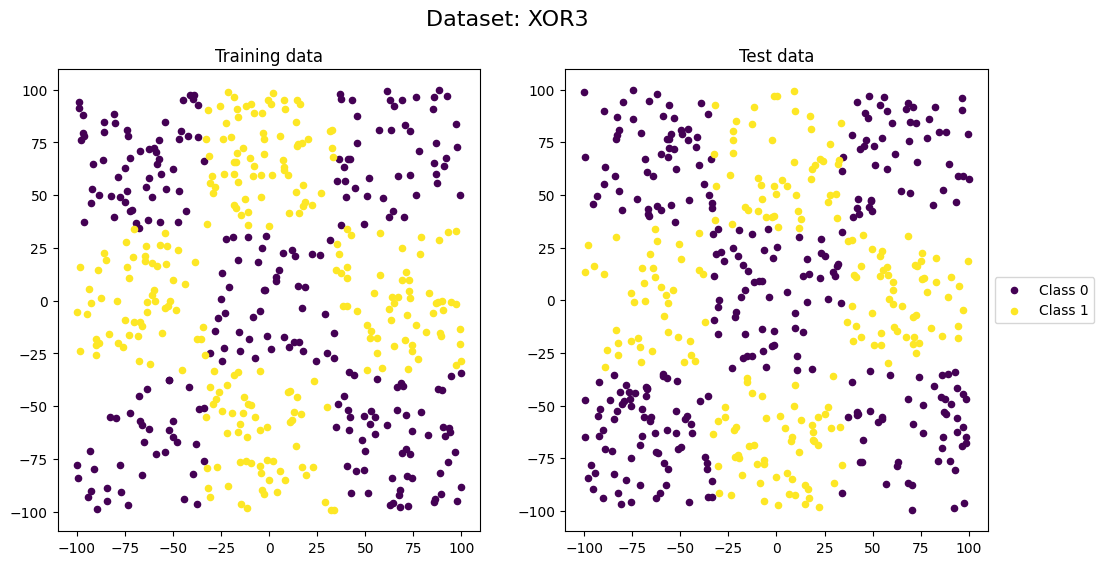
\includegraphics[width=0.7\textwidth]{img/nn4/xor3.png}
    \caption{Dataset: xor3}
\end{figure}
\newpage

\subsection*{Simple}
Ten zbiór był wyjątkowo prosty. Zarówno dla dedykowanej funkcji aktywacji \textit{Softmax}() jak i dla funkcji aktywacji \textit{Sigmoid}() model osiągnął 100\% skuteczności na zbiorze testowym. W przypadku funkcji aktywacji \textit{Softmax}() model uczył się szybciej, ale dla funkcji aktywacji \textit{Sigmoid}() model również osiągnął bardzo dobre wyniki.
\begin{figure}[H]
    \centering
    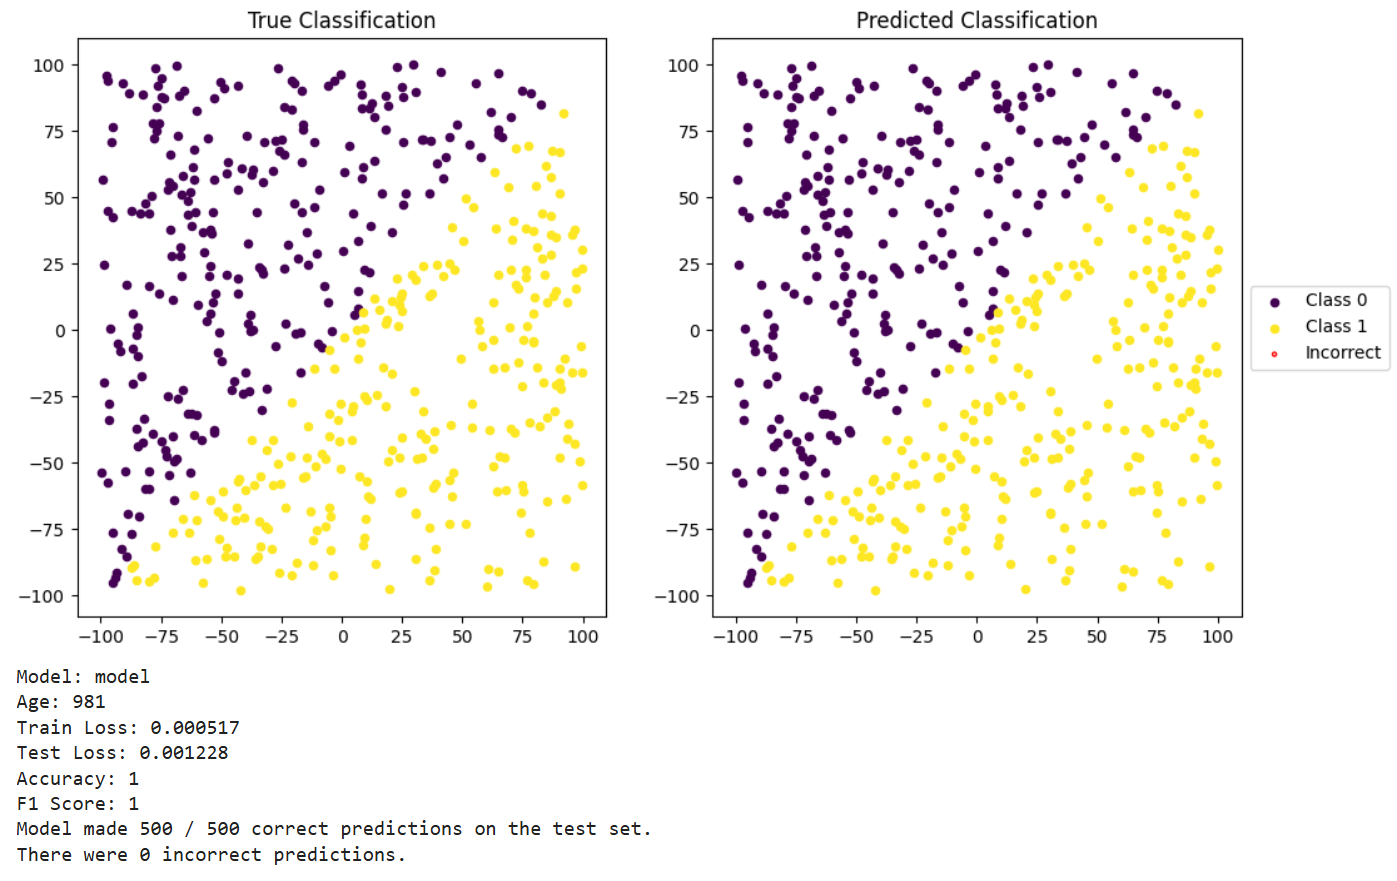
\includegraphics[width=\textwidth]{img/nn4/easy_fit.png}
    \caption{Simple: Dopasowanie modelu z obiema funkcjami dało 100\% skuteczności.} 
\end{figure}
\begin{figure}[H]
    \centering
    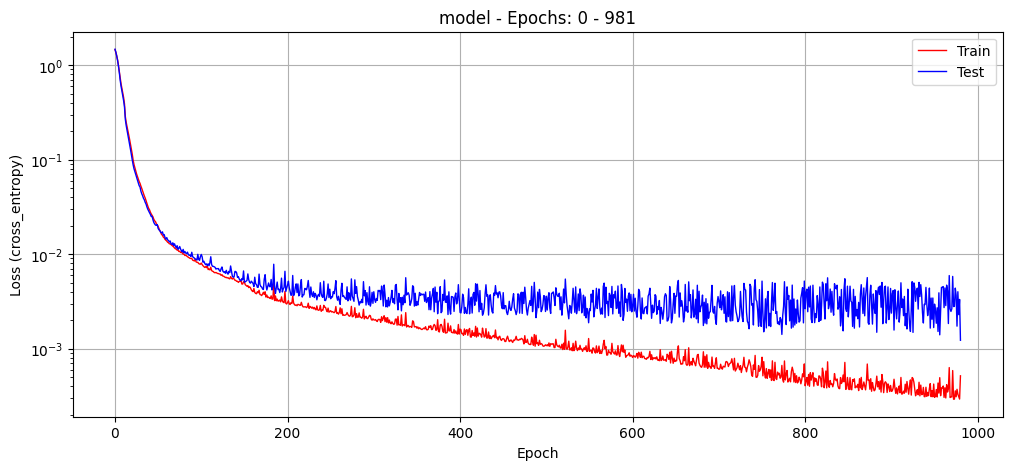
\includegraphics[width=\textwidth]{img/nn4/easy_history.png}
    \caption{Simple: Historia uczenia modelu z funkcją aktywacji Softmax} 
\end{figure}
\newpage

\subsection*{Rings3}
Ten zbiór okazał się bardziej wymagający, ale również on nie sprawił modelowi większych problemów. Model korzystający z \textit{Sigmoid}() poradził sobie nawet nieco lepiej niż model korzystający z \textit{Softmax}(), co było zadziwiające.
\begin{figure}[H]
    \centering
    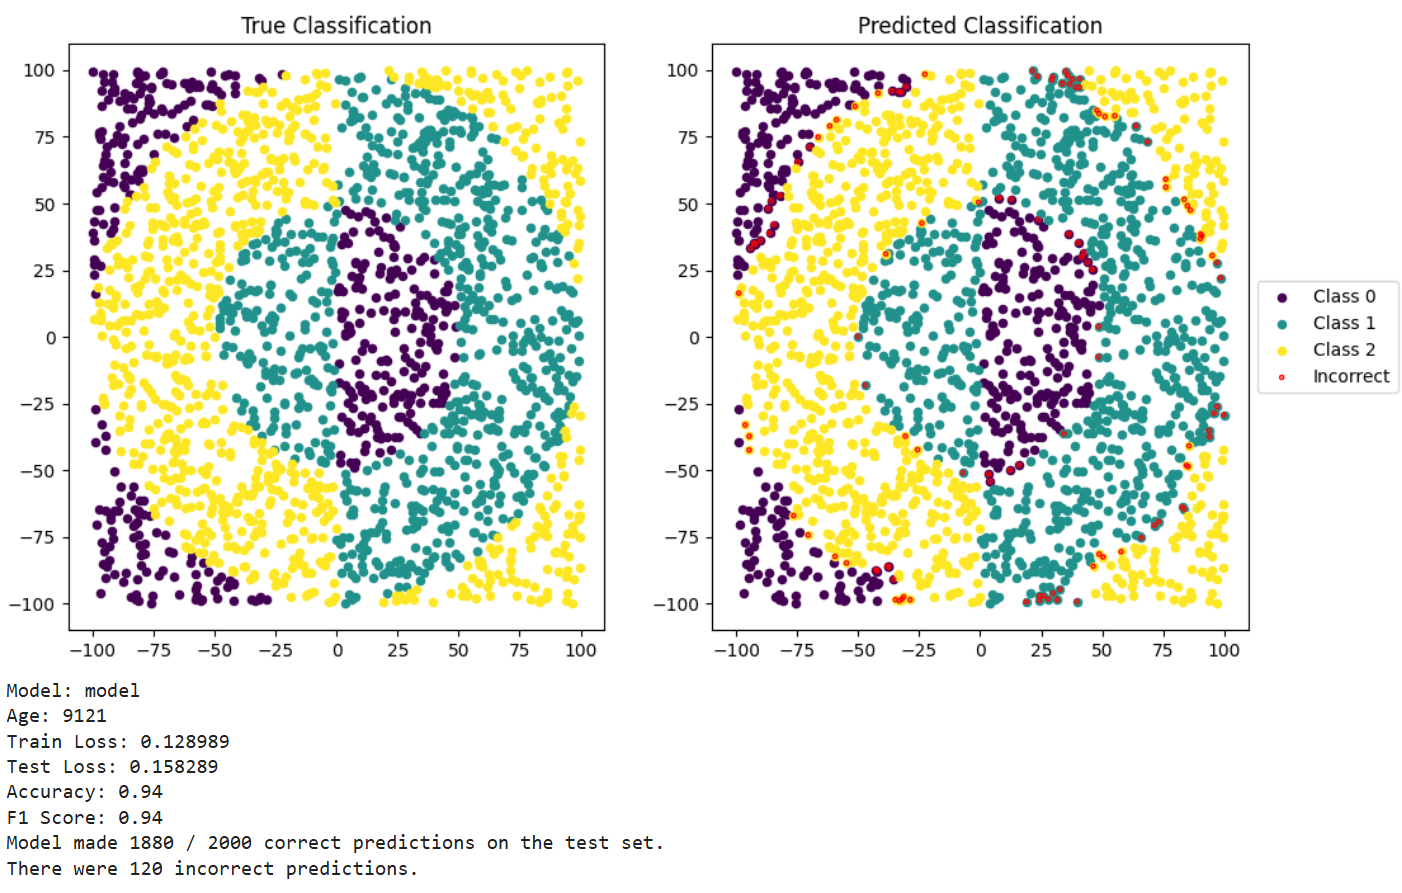
\includegraphics[width=0.95\textwidth]{img/nn4/rings3_softmax.png}
    \caption{Rings3: Dopasowanie modelu z funkcją aktywacji Softmax}
\end{figure}
\begin{figure}[H]
    \centering
    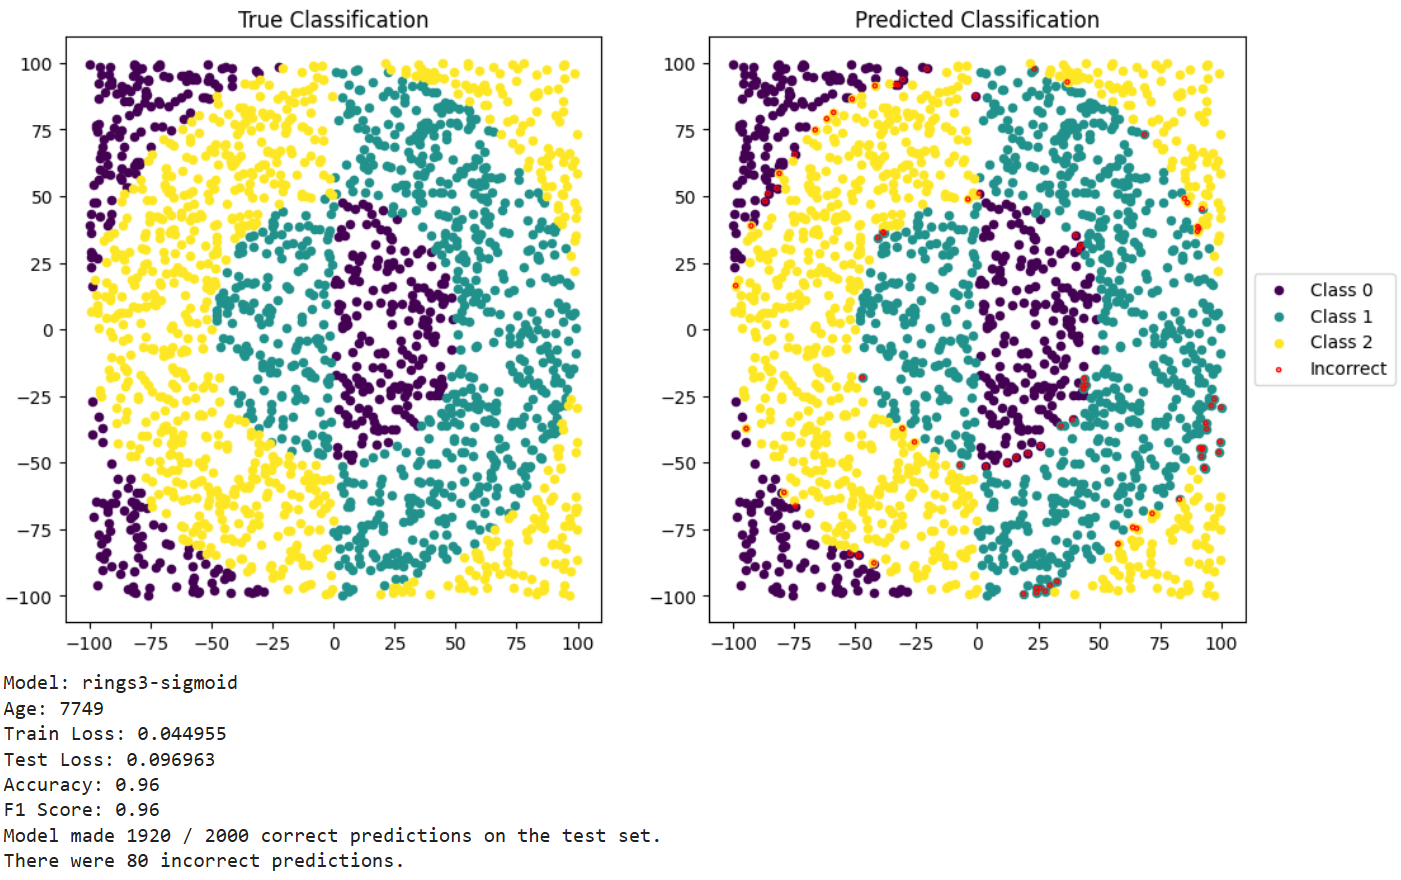
\includegraphics[width=0.95\textwidth]{img/nn4/rings3_sigmoid.png}
    \caption{Rings3: Dopasowanie modelu z funkcją aktywacji Sigmoid} 
\end{figure}
\newpage

\subsection*{Xor3}
Zbiór xor3 również okazał się dosyć prosty. Jakość predykcji modeli w obu przypadkach była bardzo bardzo dobra, nieco lepsza dla Softmaxa.
\begin{figure}[H]
    \centering
    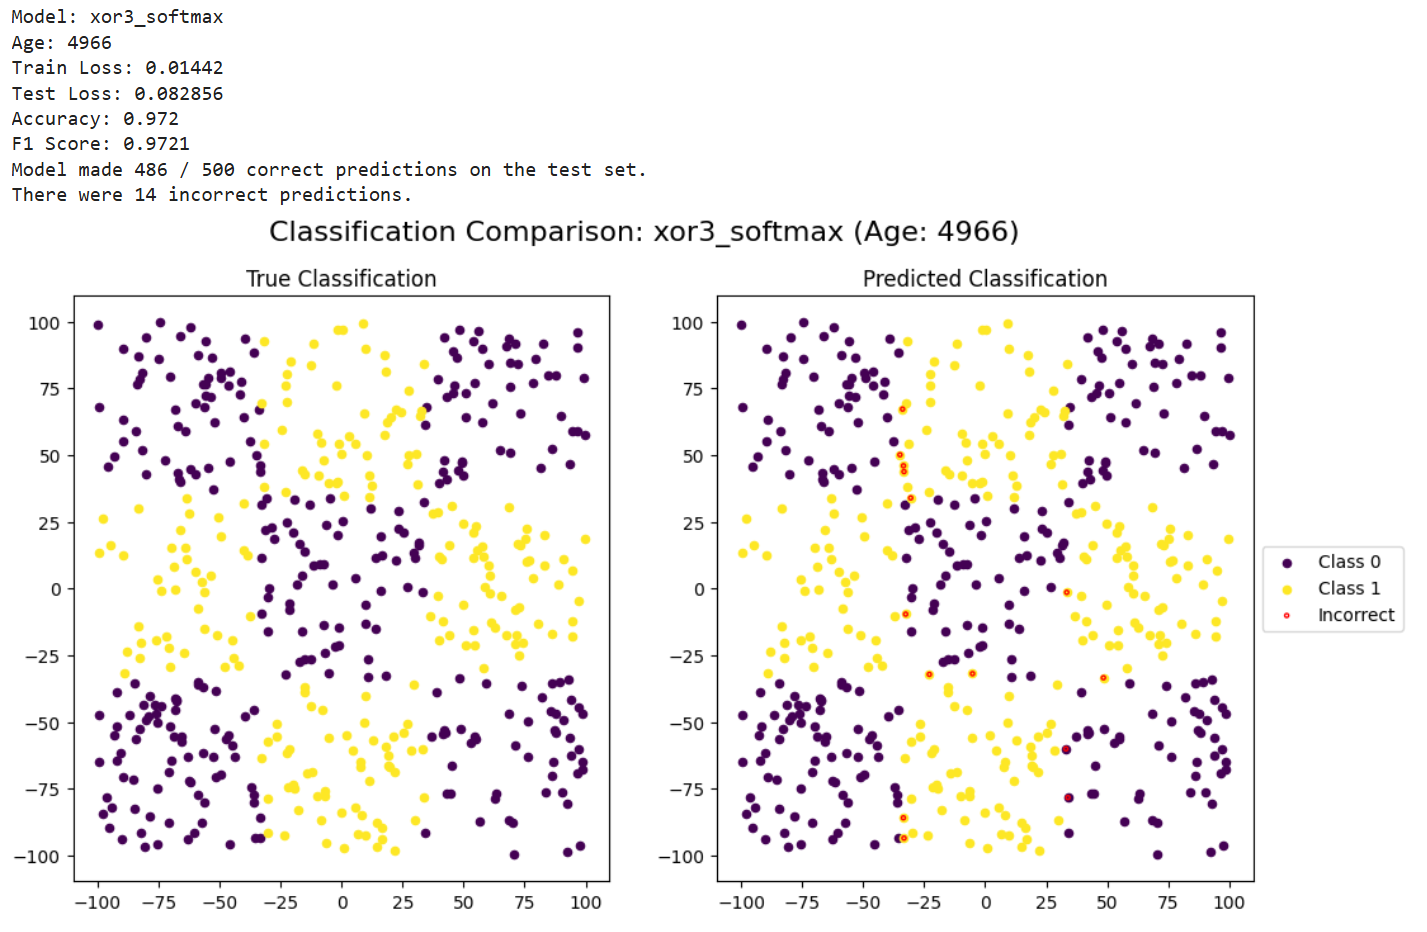
\includegraphics[width=0.95\textwidth]{img/nn4/xor3_softmax.png}
    \caption{Xor3: Dopasowanie modelu z funkcją aktywacji Softmax}
\end{figure}
\begin{figure}[H]
    \centering
    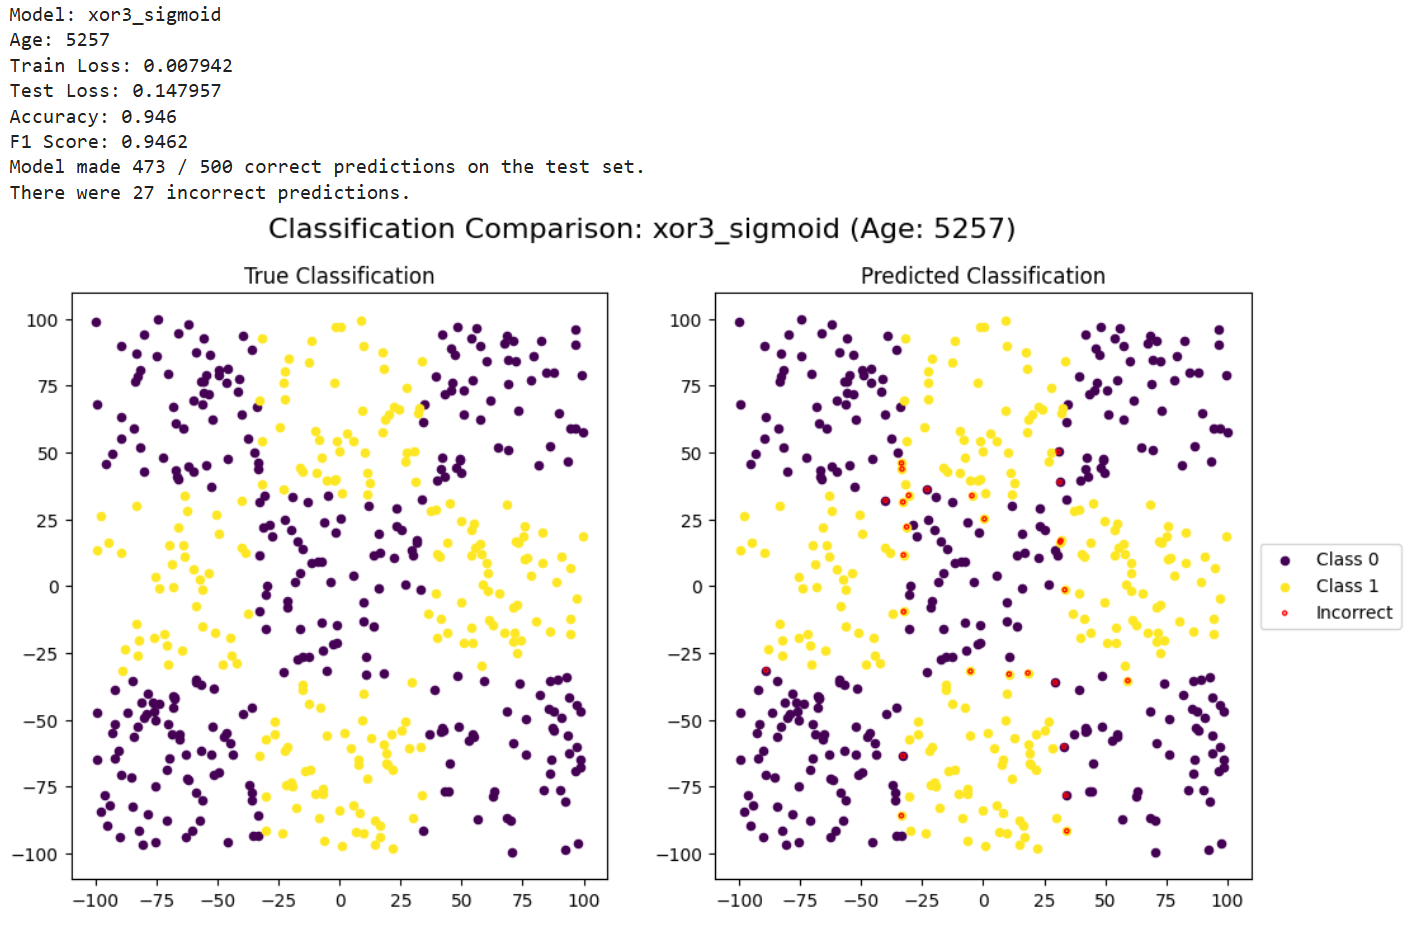
\includegraphics[width=0.95\textwidth]{img/nn4/xor3_sigmoid.png}
    \caption{Xor3: Dopasowanie modelu z funkcją aktywacji Sigmoid}
\end{figure}


\section*{NN5: Testowanie różnych funkcji aktywacji}
\addcontentsline{toc}{section}{NN5: Testowanie różnych funkcji aktywacji}
\subsection*{Cel}
\begin{enumerate}
    \item[a)] Przetestowanie różnych kombinacji architektur i funkcji aktywacji w sieciach neuronowych, takich jak ReLU, tanh, sigmoid, funkcja liniowa oraz ich wpływu na proces uczenia i jakość predykcji.
    \item[c)] Szczegółowe testy dla 2 najlepszych kombinacji na zbiorach:
    \item[] \begin{itemize}
        \item steps-large
        \item rings5-regular
        \item rings3-regular
    \end{itemize}
\end{enumerate}

\subsection*{Funkcje aktywacji i ich pochodne}
Testowane były 4 funkcje aktywacji:
\begin{figure}[H]
    \centering
    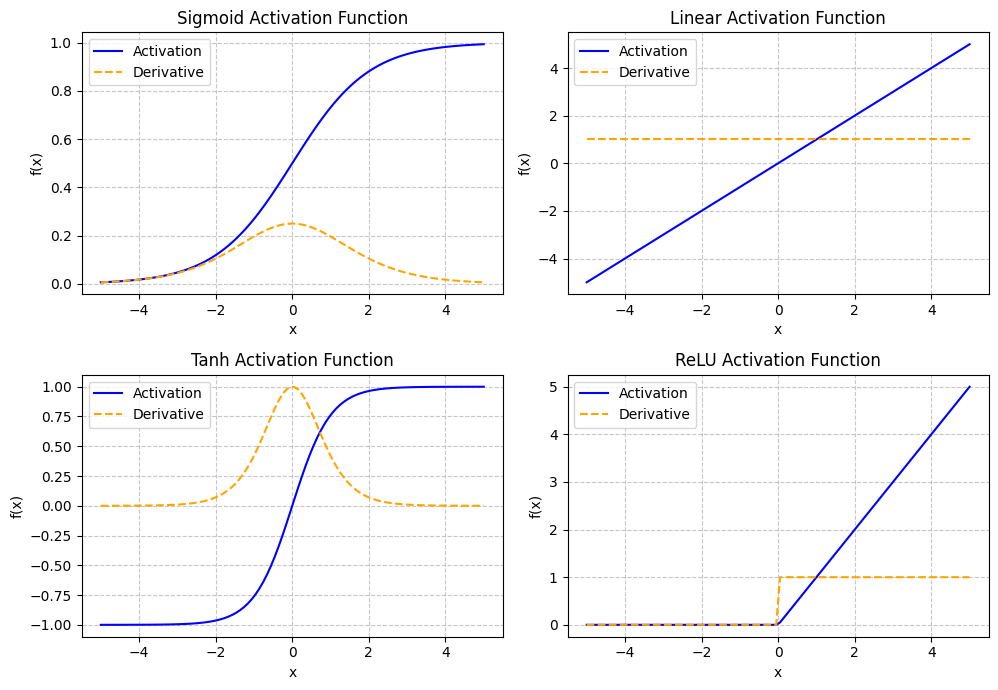
\includegraphics[width=\textwidth]{img/nn5/pochodne.png}
    \caption{Funkcje aktywacji i ich pochodne}
\end{figure}

\subsection*{Architektury}
Testowane były 3 architektury, z 1, 2 oraz 3 warstwami ukrytymi. Każda architektura dzieliła między warstwy 80 neuronów:
\begin{itemize}
    \item \textbf{1-80-1}
    \item \textbf{1-40-40-1}
    \item \textbf{1-20-40-20-1}
\end{itemize}

\subsection*{Wstępne testy}
Wstępne testy przeprowadzono na zbiorze \textit{multimodal-large}. 
\begin{figure}[H]
    \centering
    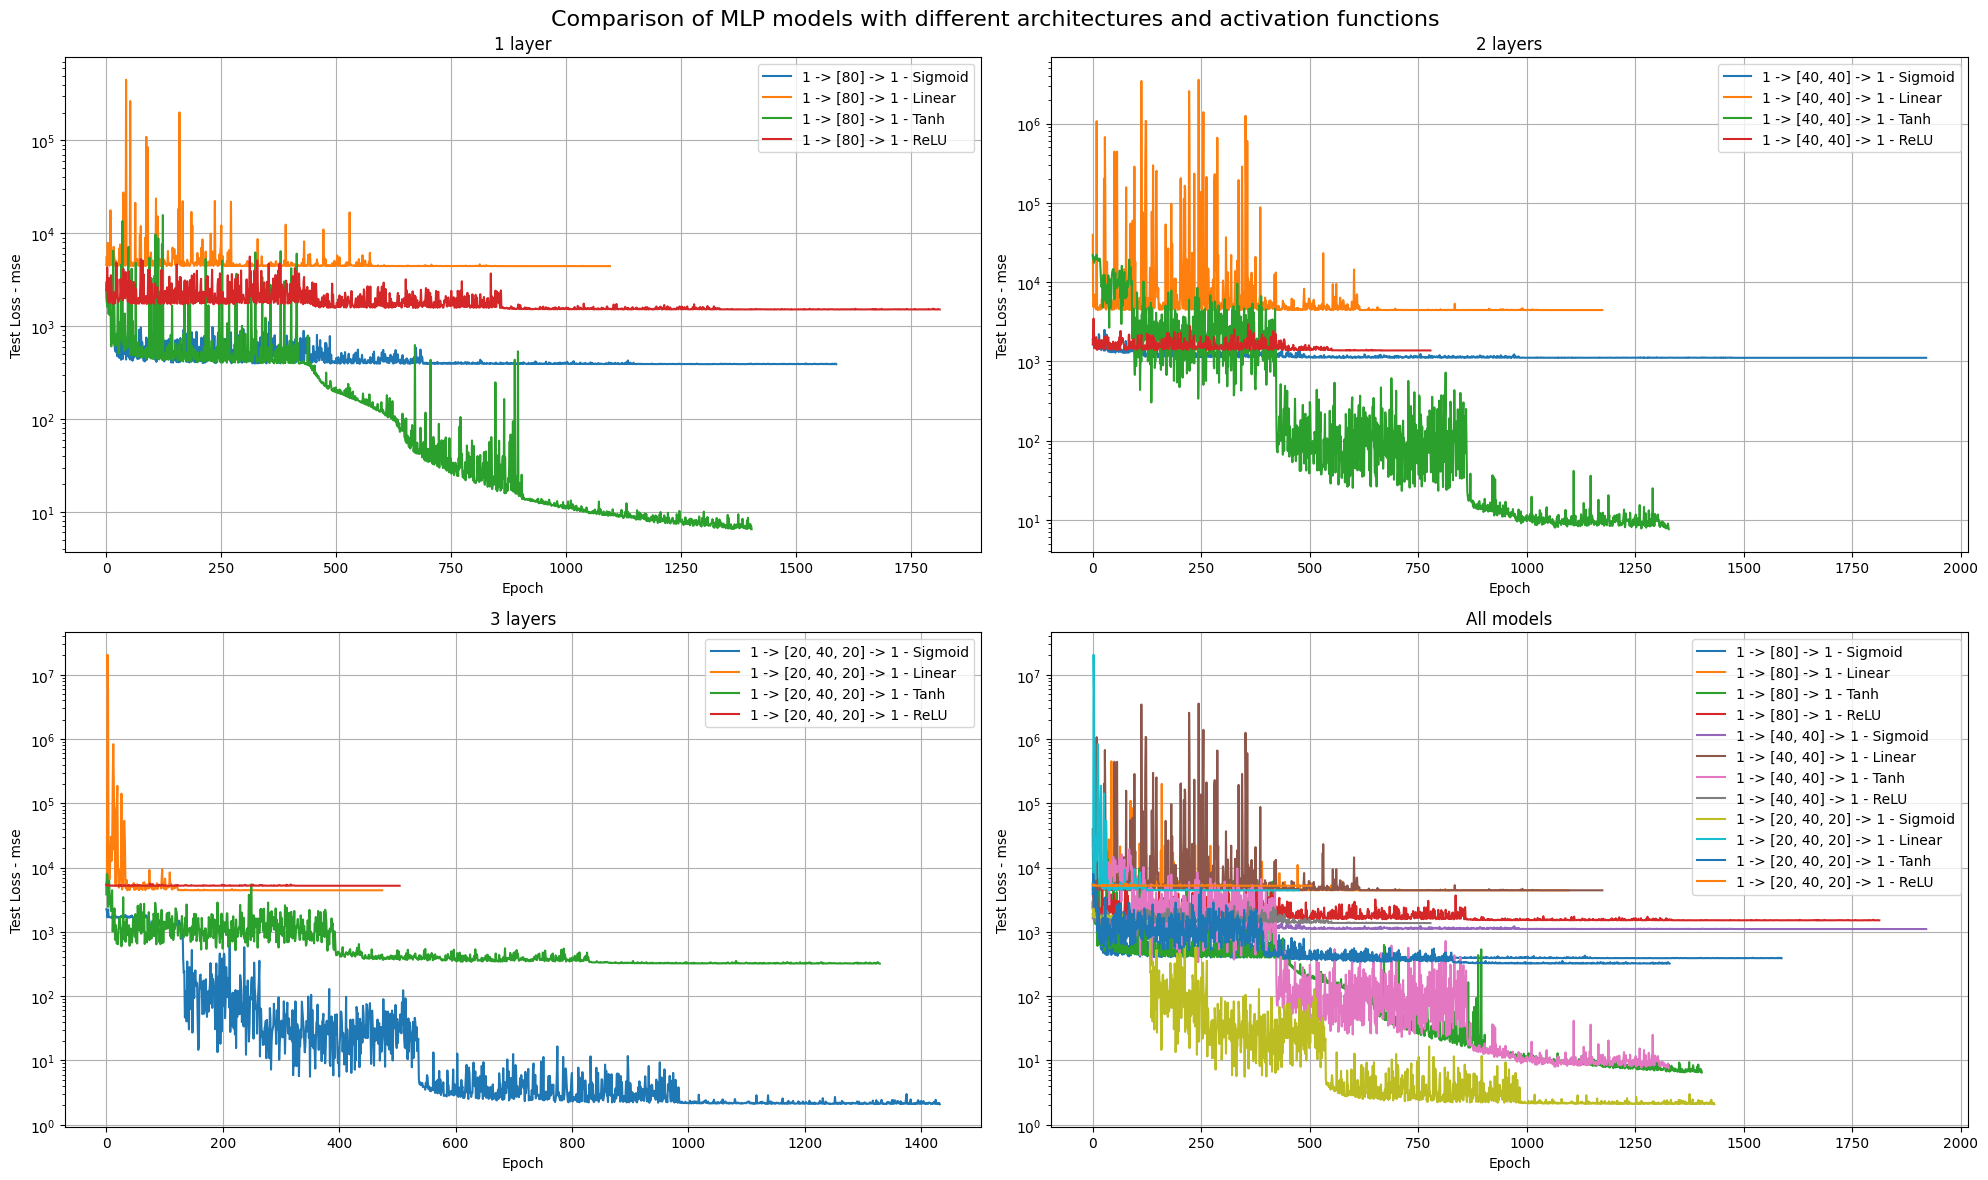
\includegraphics[width=\textwidth]{img/nn5/kombinacje.png}
    \caption{Różne kombinacje architektur i funkcji aktywacji}
\end{figure}
\subsubsection*{Wnioski}
\begin{itemize}
    \item Najlepsze wyniki osiągają modele z funkcją aktywacji \textbf{tanh} oraz \textbf{sigmoid}.
    \item Funkcja aktywacji \textbf{sigmoid} najlepiej funkcjonuje przy bardziej złożonej architekturze.
    \item W przypadku funkcji \textbf{tanh} zwiększenie liczby warstw architektury wpłynęło negatywnie na osiągnięty wynik. Najlepsze rezultaty uzyskano już przy 1 lub 2 warstwach.
\end{itemize}

Można wyróżnić 3 konkurencyjne modele:
\begin{itemize}
    \item \textbf{1-80-1} z funkcją aktywacji \textbf{tanh}
    \item \textbf{1-40-40-1} z funkcją aktywacji \textbf{tanh}
    \item \textbf{1-20-40-20-1} z funkcją aktywacji \textbf{sigmoid}
\end{itemize}
Te właśnie modele będą testowane na kolejnych zbiorach.

\subsection*{Wyniki dla zbioru rings3-regular}
\begin{figure}[H]
    \centering
    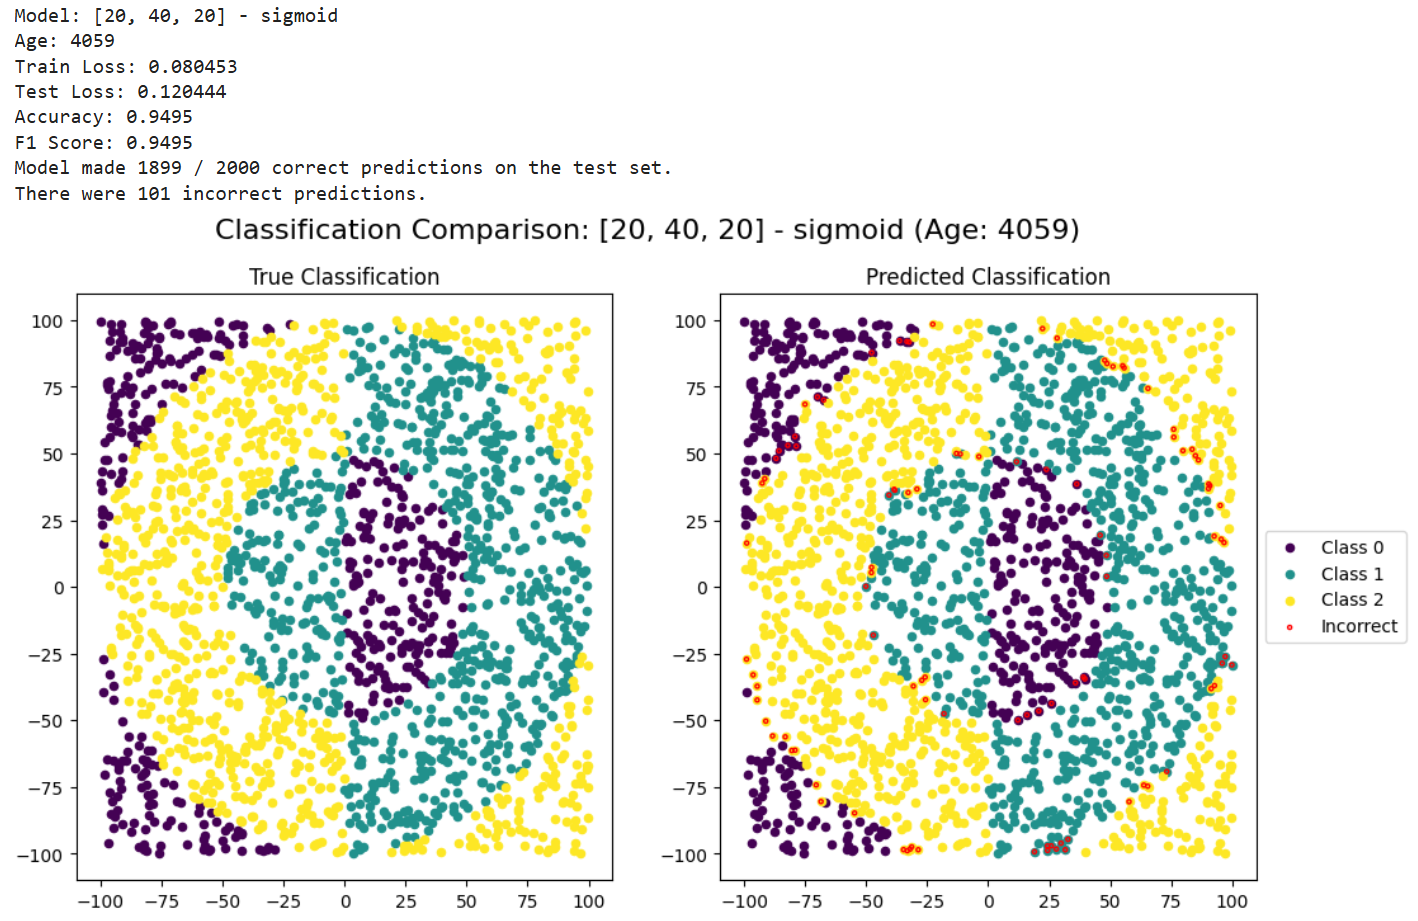
\includegraphics[width=\textwidth]{img/nn5/rings3_fit.png}
    \caption{Dopasowanie modeli do zbioru rings3-regular}
\end{figure}
\begin{figure}[H]
    \centering
    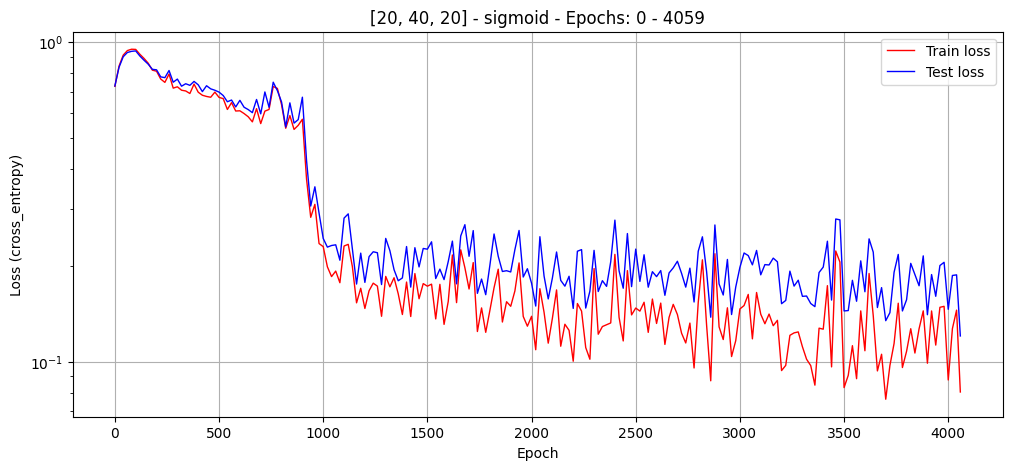
\includegraphics[width=\textwidth]{img/nn5/rings3_history.png}
    \caption{Historia uczenia modeli na zbiorze rings3-regular (cross\_entropy)}
\end{figure}

Wszystkie trzy testowane modele:
\begin{itemize}
    \item \textbf{1-80-1} z funkcją aktywacji \textbf{tanh}
    \item \textbf{1-40-40-1} z funkcją aktywacji \textbf{tanh}
    \item \textbf{1-20-40-20-1} z funkcją aktywacji \textbf{sigmoid}
\end{itemize}
uzyskały bardzo zbliżone wyniki na zbiorze \textit{rings3-regular}. Każdy z modeli osiągnął wartość F1-score na poziomie około 0{,}95 po 3000--5000 epokach treningu. Dalsze zwiększanie liczby epok nie przynosiło już istotnej poprawy jakości predykcji.

\begin{center}
\begin{tabular}{|c|c|c|}
    \hline
    Architektura & Funkcja aktywacji & F1-score \\
    \hline
    1-80-1 & tanh & 0,9476 \\
    1-40-40-1 & tanh & 0,9475 \\
    1-20-40-20-1 & sigmoid & 0,9495 \\
    \hline
\end{tabular}
\end{center}

Wnioski: wszystkie testowane konfiguracje sieci neuronowych pozwalają na skuteczne rozwiązanie zadania klasyfikacji na tym zbiorze danych.

\subsection*{Wyniki dla zbioru rings5-regular}
\begin{figure}[H]
    \centering
    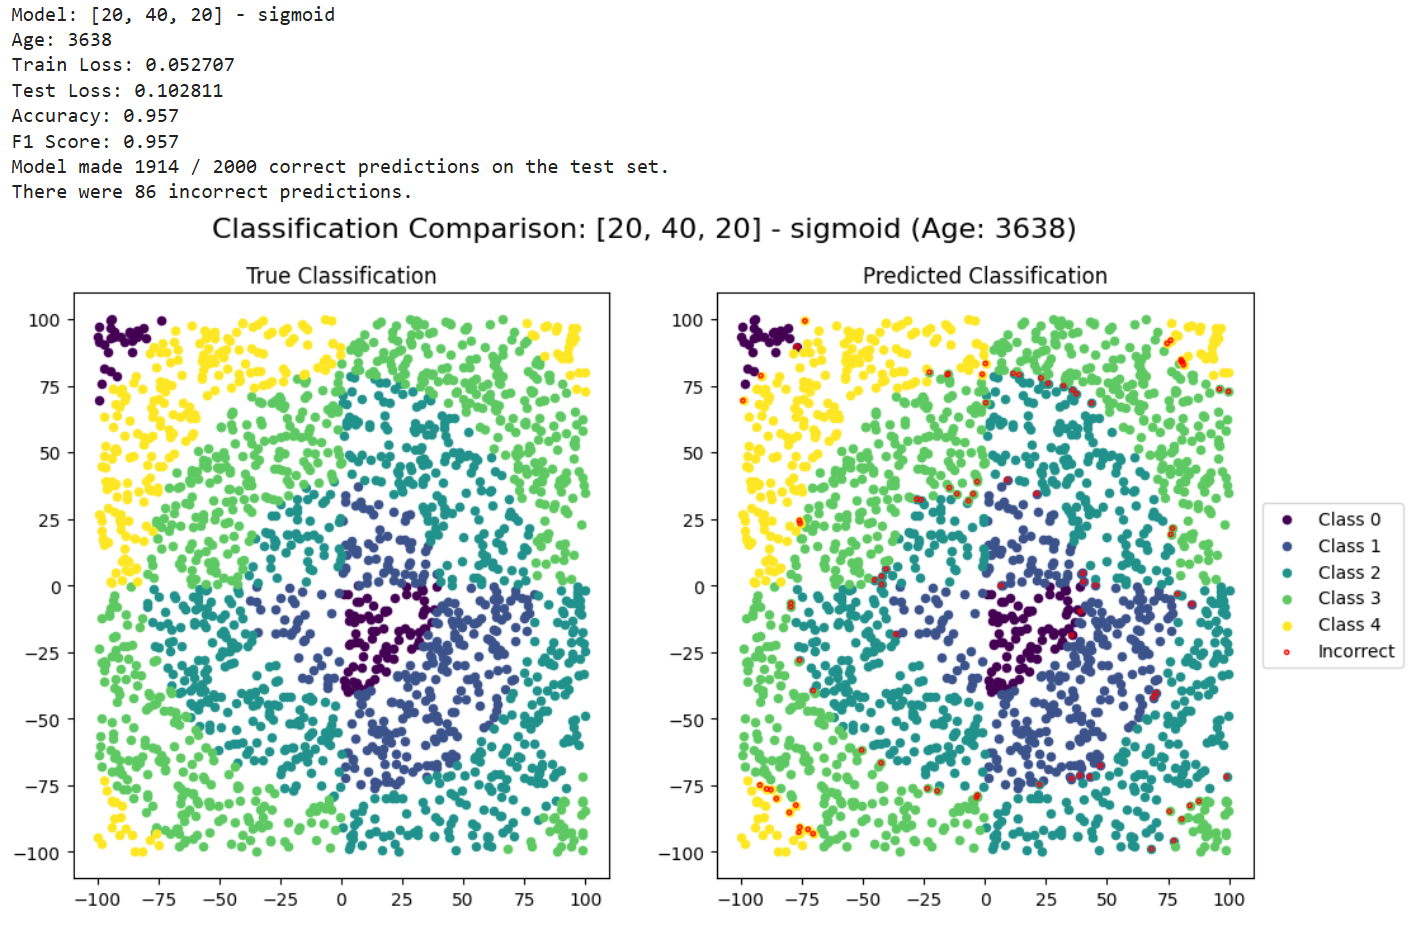
\includegraphics[width=0.9\textwidth]{img/nn5/rings5_fit.png}
    \caption{Dopasowanie modelu do zbioru rings5-regular}
\end{figure}
\begin{figure}[H]
    \centering
    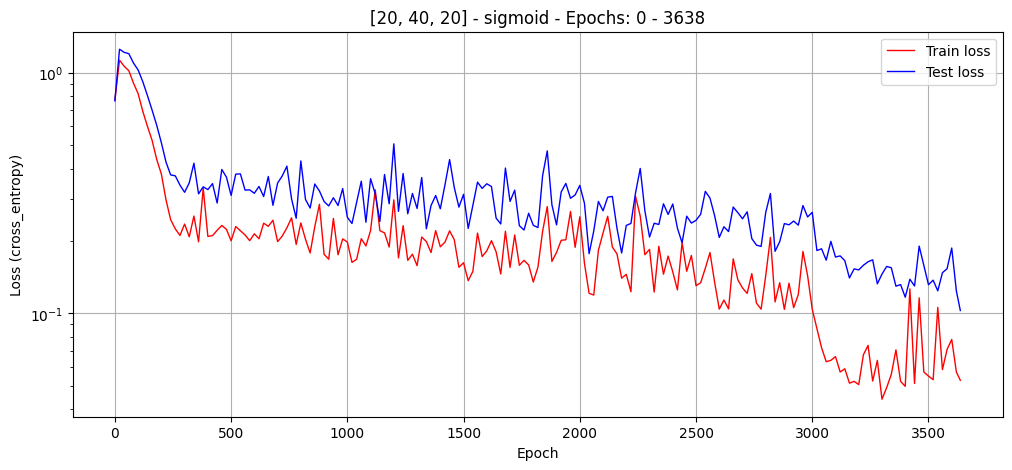
\includegraphics[width=0.9\textwidth]{img/nn5/rings5_history.png}
    \caption{Historia uczenia modelu na zbiorze rings5-regular (cross\_entropy)}
\end{figure}


Zdecydowanie najlepszy okazał się model \textbf{1-20-40-20-1} z funkcją aktywacji \textbf{sigmoid}, który osiągnął wartość F1-score na poziomie około 0{,}957 po 3638 epokach treningu.

\begin{center}
\begin{tabular}{|c|c|c|}
    \hline
    Architektura & Funkcja aktywacji & F1-score \\
    \hline
    1-80-1 & tanh & 0,9178 \\
    1-40-40-1 & tanh & 0,9339 \\
    1-20-40-20-1 & sigmoid & 0,957 \\
    \hline
\end{tabular}
\end{center}

Wszystkie modele pozwalają na rozwiązanie zadania klasyfikacji na tym zbiorze danych, jednak model z funkcją aktywacji \textit{sigmoid} okazał się zdecydowanie najlepszy.

\subsection*{Wyniki dla zbioru steps-large}
\begin{figure}[H]
    \centering
    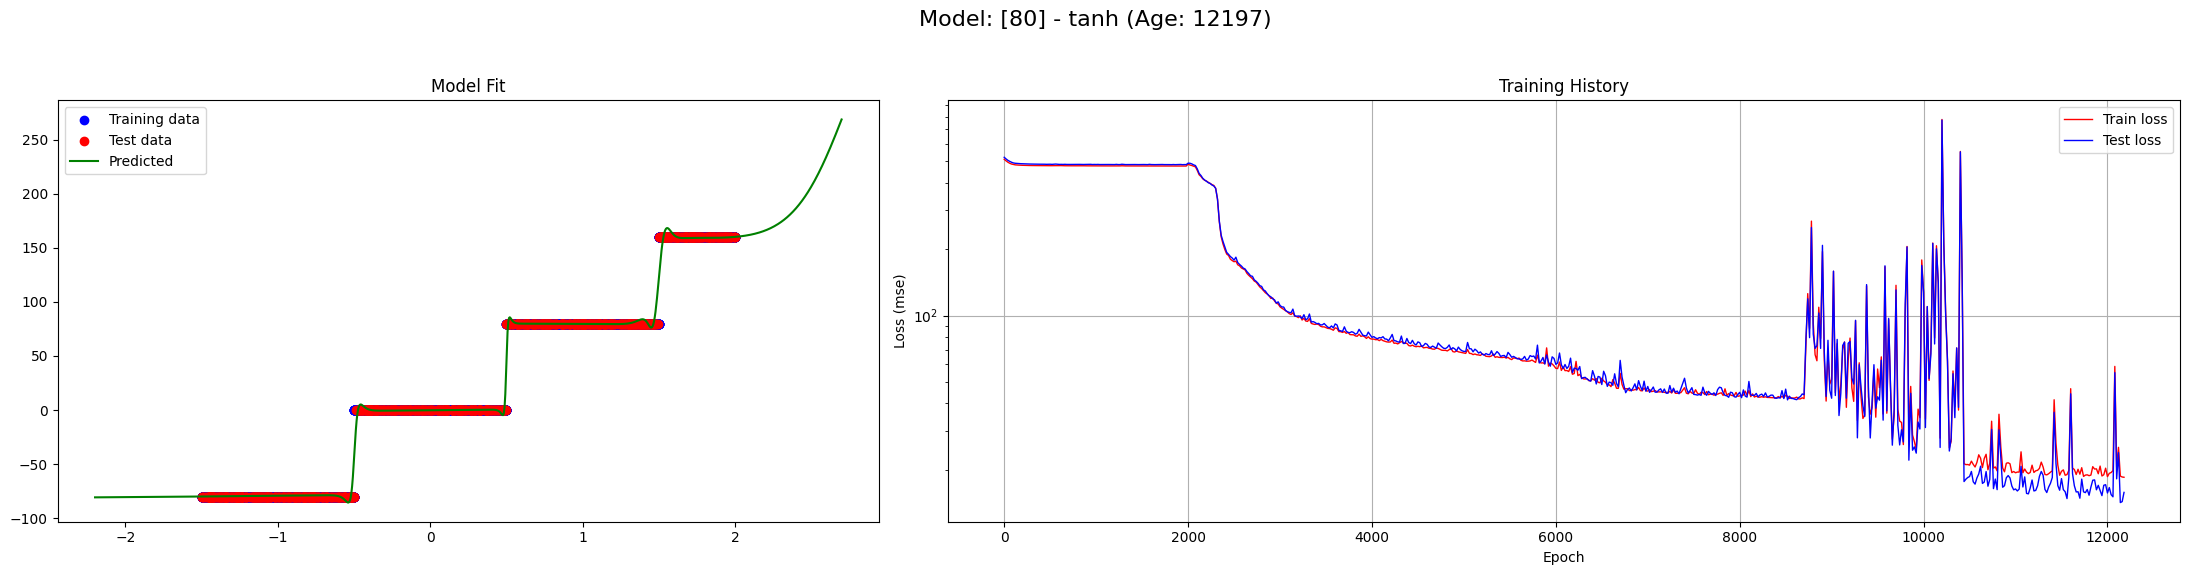
\includegraphics[width=\textwidth]{img/nn5/steps-large_tanhsimple.png}
    \caption{Dopasowanie oraz historia uczenia (log(MSE)) modelu z funkcją aktywacji \textbf{tanh} oraz jedną warstwą ukrytą \textbf{(1-80-1)}}
\end{figure}
\begin{figure}[H]
    \centering
    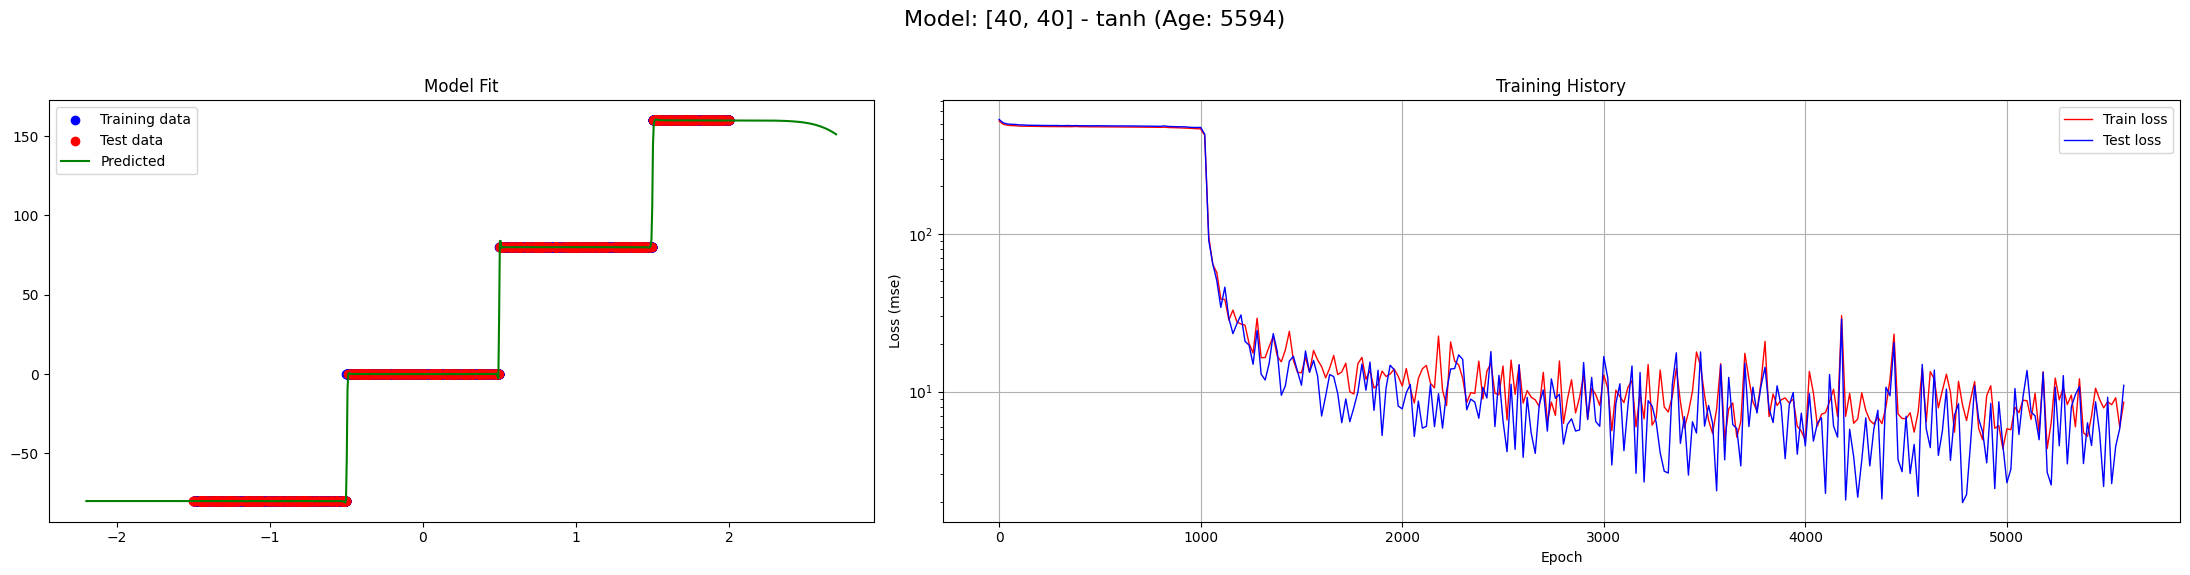
\includegraphics[width=\textwidth]{img/nn5/steps-large_tanh.png}
    \caption{Dopasowanie oraz historia uczenia (log(MSE)) modelu z funkcją aktywacji \textbf{tanh} oraz dwiema warstwami ukrytymi \textbf{(1-40-40-1)}}
\end{figure}
\begin{figure}[H]
    \centering
    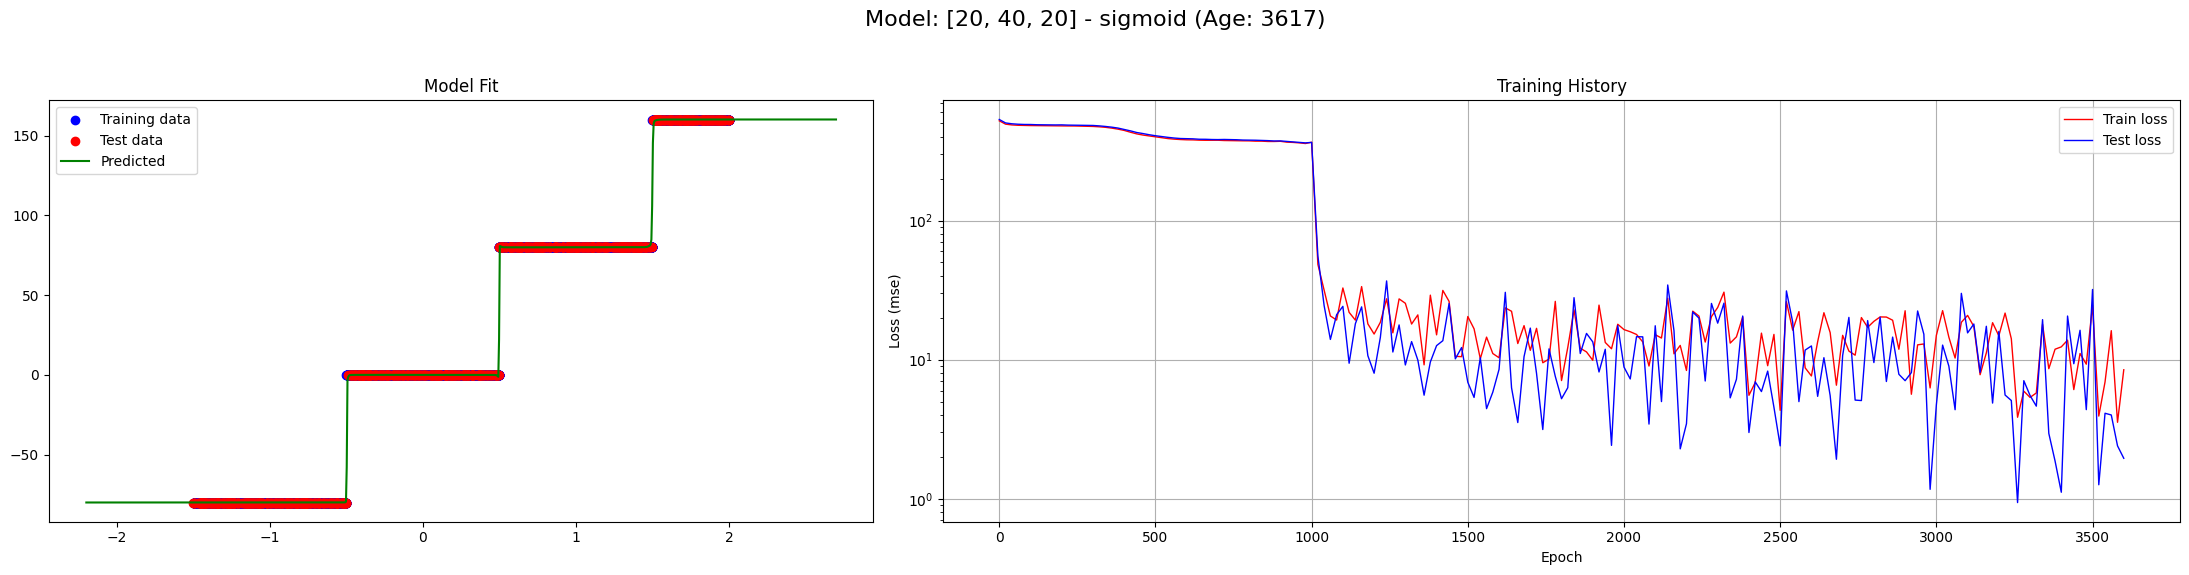
\includegraphics[width=\textwidth]{img/nn5/steps-large_sigmoid.png}
    \caption{Dopasowanie oraz historia uczenia (log(MSE)) modelu z funkcją aktywacji \textbf{sigmoid}}
\end{figure}

\begin{center}
\begin{tabular}{|c|c|c|c|c|}
    \hline
    Architektura & Funkcja aktywacji & Liczba epok & MSE (train) & MSE (test) \\
    \hline
    1-80-1 & tanh & 12197 & 18.57 & 14.09 \\
    1-40-40-1 & tanh & 5594 & 6.56 & 1.44 \\
    1-20-40-20-1 & sigmoid & 3617 & 6.24 & 0.48 \\
    \hline
\end{tabular}
\end{center}

\subsubsection*{Wnioski}
Wszystkie modele poradziły sobie z zadaniem na przyzwoitym poziomie.

Model \textbf{1-80-1} z funkcją aktywacji \textbf{tanh} ze względu na prostą architekturę miał trudności z dokładnym odwzorowaniem przejść pomiędzy stopniami w zbiorze \textit{steps-large}.

Modele \textbf{1-40-40-1} z funkcją \textbf{tanh} oraz \textbf{1-20-40-20-1} z funkcją \textbf{sigmoid} osiągnęły lepsze wyniki (MSE na poziomie około 1), szczególnie dobrze radząc sobie z odwzorowaniem miejsc przejść. Głębsze architektury oraz odpowiedni dobór funkcji aktywacji pozwoliły lepiej uchwycić złożoność zbioru danych. Ogólnie, zwiększenie głębokości modelu oraz tuning funkcji aktywacji poprawiły rezultaty na zbiorze \textit{steps-large}.

\section*{NN6: Regularyzacja i przeuczanie}
\addcontentsline{toc}{section}{NN6: Regularyzacja i przeuczanie}
\subsection*{Cel}
\begin{enumerate}
    \item[a)] Zaimplementowanie mechanizmów regularyzacji w sieciach neuronowych, takich jak L1 oraz L2 w celu ograniczenia przeuczania.
    \item[b)] Przeprowadzenie eksperymentów porównujących skuteczność regularyzacji na wybranych zbiorach danych, ze szczególnym uwzględnieniem wpływu na generalizację modelu.
\end{enumerate}

\subsection*{Implementacja}
Na tym etapie do implementacji zostały dodane następujące mechanizmy regularyzacji:
\begin{itemize}
    \item \textbf{Regularyzacja L1 oraz L2} -- umożliwiająca ograniczenie wartości wag w sieci neuronowej, co pozwala na redukcję ryzyka przeuczania. Współczynniki regularyzacji można ustawić osobno dla \texttt{L1} i \texttt{L2}, co zapewnia elastyczność w doborze odpowiedniej metody do konkretnego zadania.
    \item \textbf{Parametr \texttt{save\_till\_best}} w funkcji \texttt{train()} -- umożliwia automatyczne zapisywanie najlepszego modelu (na podstawie wyniku na zbiorze testowym) podczas procesu uczenia oraz przywrócenie tych parametrów po zakończeniu treningu. Takie podejście pozwala na uniknięcie sytuacjim, w której model osiąga coraz lepsze wyniki na zbiorze treningowym, ale gorsze na zbiorze testowym, co jest typowym objawem przeuczania.
\end{itemize}

\section*{Wyniki}

Dla zadań klasyfikacyjnych regularyzacja nie przyniosła pożądanych rezultatów. W przypadku zbiorów \textit{rings3-regular} oraz \textit{rings5-regular} modele z regularyzacją L1 oraz L2 osiągnęły gorsze lub takie same wyniki niż modele bez regularyzacji. Dla zbioru \textit{xor3-balance} regularyzacja poprawiła wyniki. \\
\\
Model bez regularyzacji osiągał F1-score na poziomie 0.88, podczas gdy model z regularyzacją L2 osiągnął F1-score na poziomie 0.93

\begin{figure}[H]
    \centering
    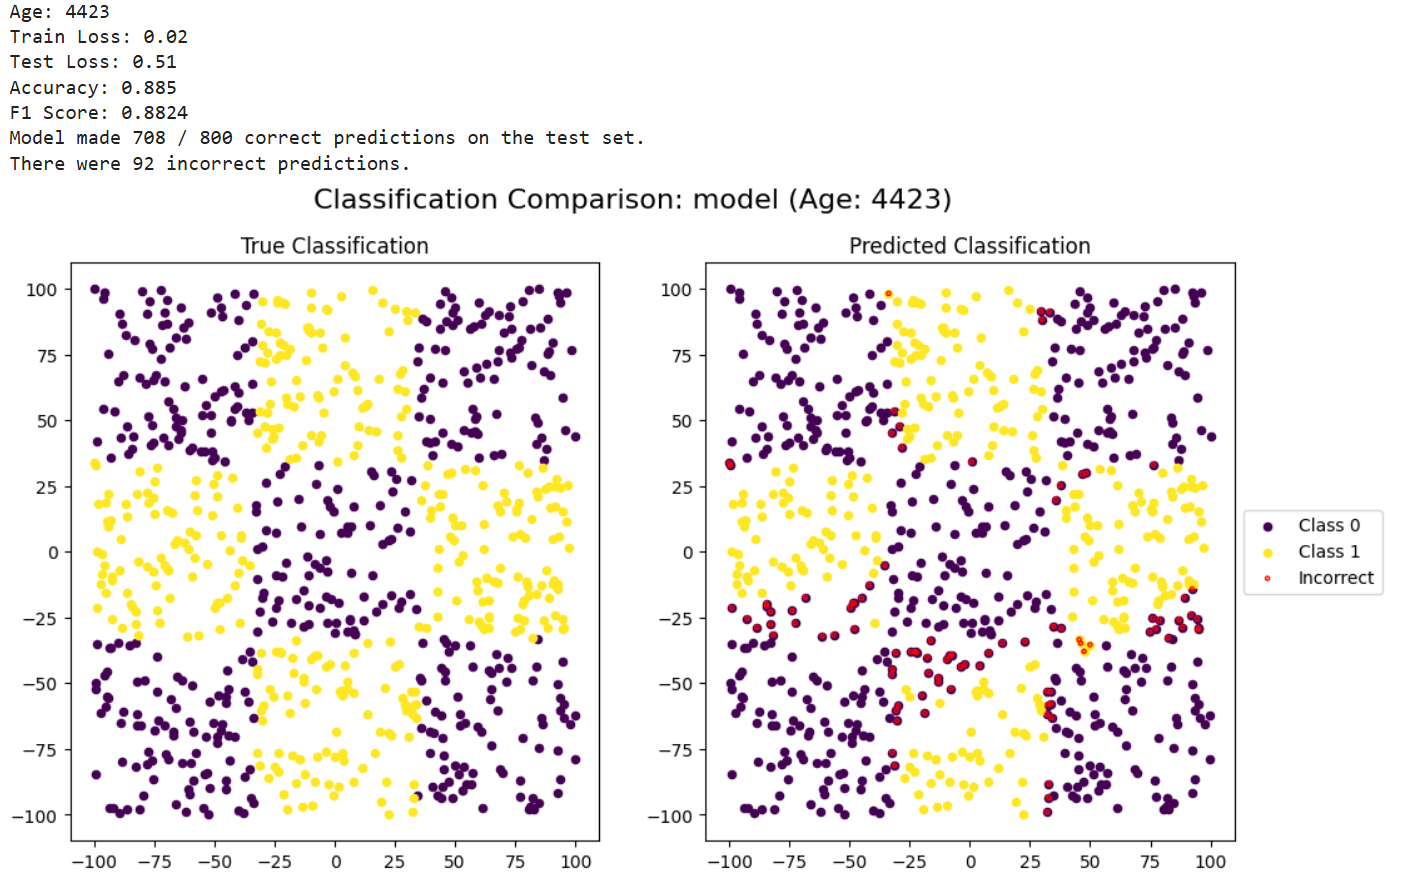
\includegraphics[width=0.7\textwidth]{img/nn6/xor_noreg.png}
    \caption{Dopasowanie modelu bez regularyzacji do zbioru xor3-balance}
\end{figure}

\begin{figure}[H]
    \centering
    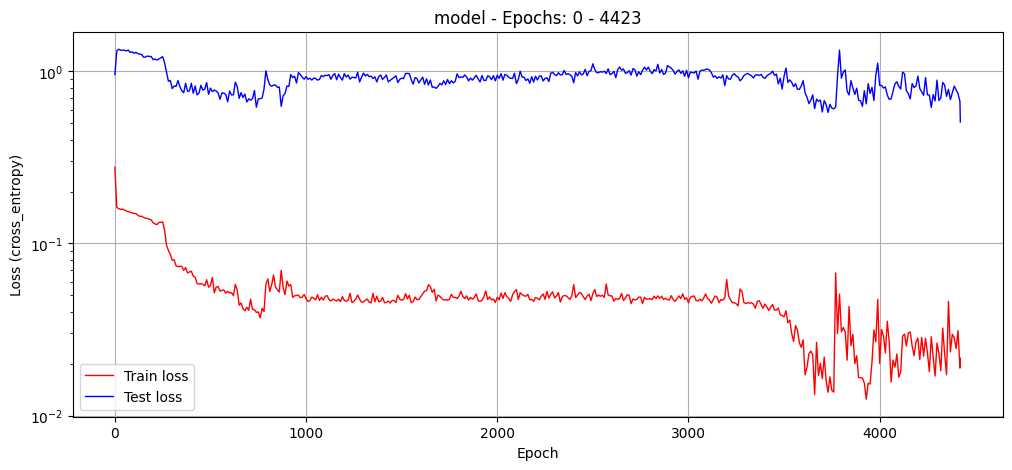
\includegraphics[width=0.7\textwidth]{img/nn6/xor_noreg_hist.png}
    \caption{Historia uczenia modelu bez regularyzacji na zbiorze xor3-balance}
\end{figure}

\begin{figure}[H]
    \centering
    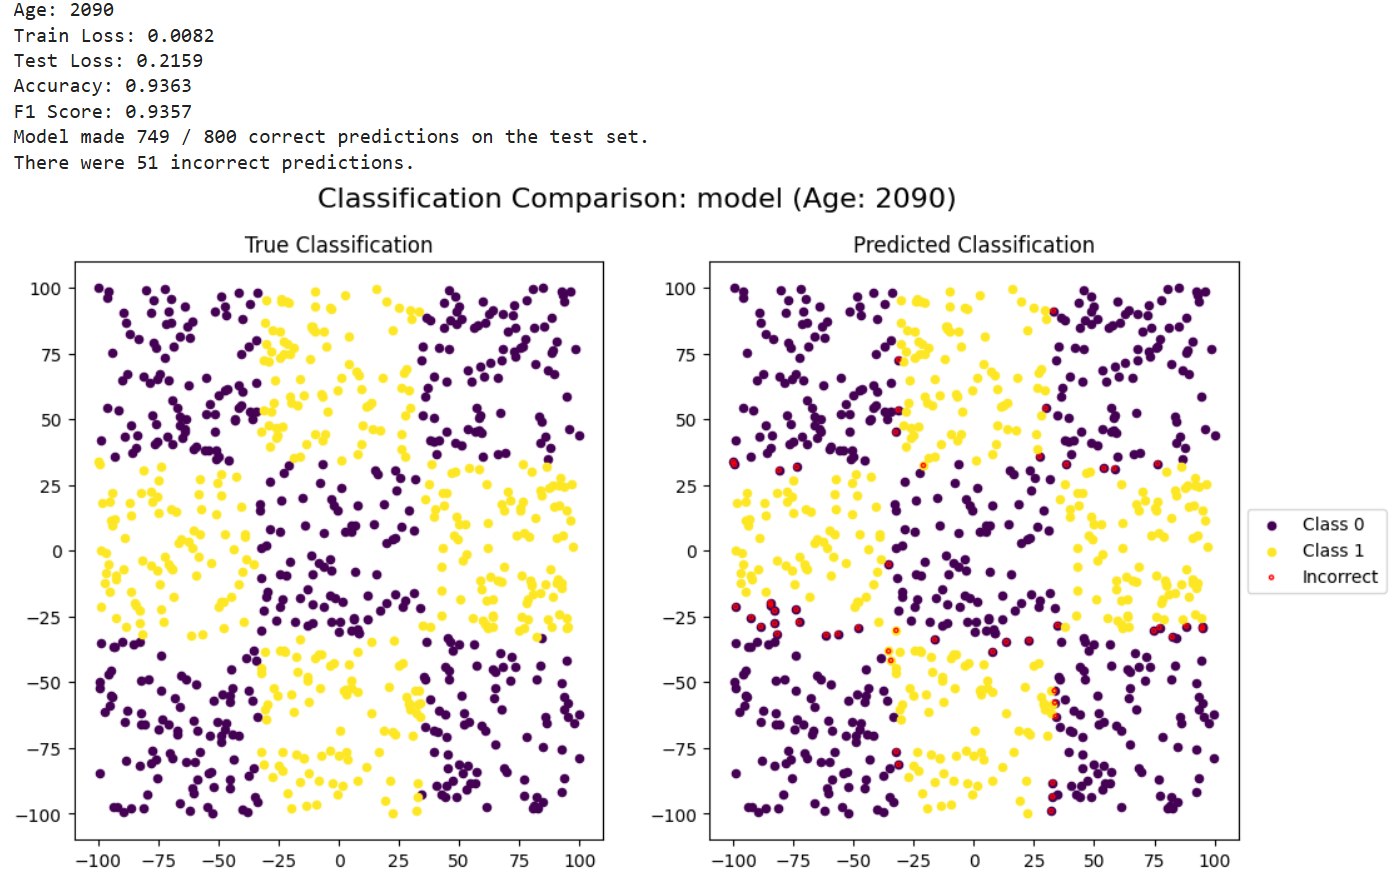
\includegraphics[width=0.7\textwidth]{img/nn6/xor_reg.png}
    \caption{Dopasowanie modelu z regularyzacją L1 do zbioru xor3-balance}
\end{figure}

\begin{figure}[H]
    \centering
    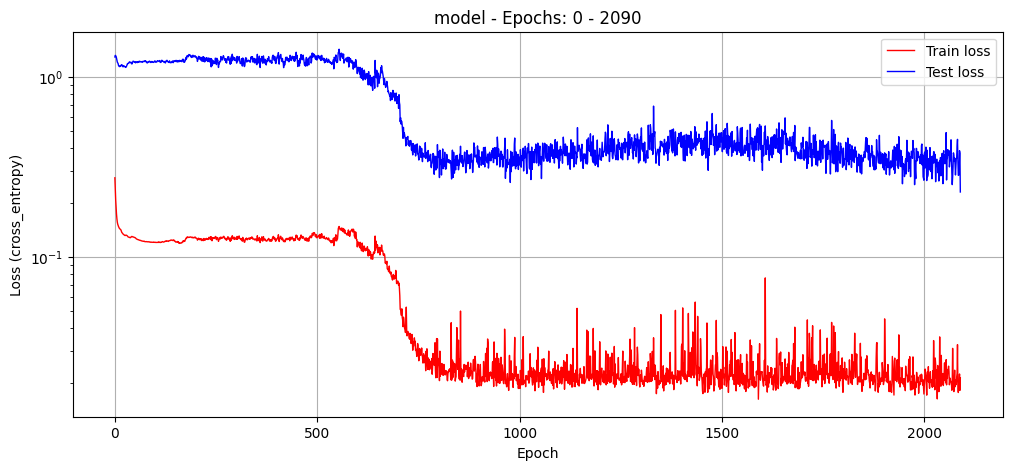
\includegraphics[width=0.7\textwidth]{img/nn6/xor_reg_hist.png}
    \caption{Wpływ regularyzacji L1 na zbiór xor3-balance}
\end{figure}

\subsubsection*{Największy sukces}
Najlepsze rezultaty udało się osiągnąć na zbiorze \textit{multimodal-sparse} przy użyciu regularyzacji L2. Model z regularyzacją L2 osiągnął MSE na poziomie 5.5 na zbiorze testowym, co jest znaczącą poprawą w porównaniu do modelu bez regularyzacji, który osiągnął MSE na poziomie 50.72.

\begin{figure}[H]
    \centering
    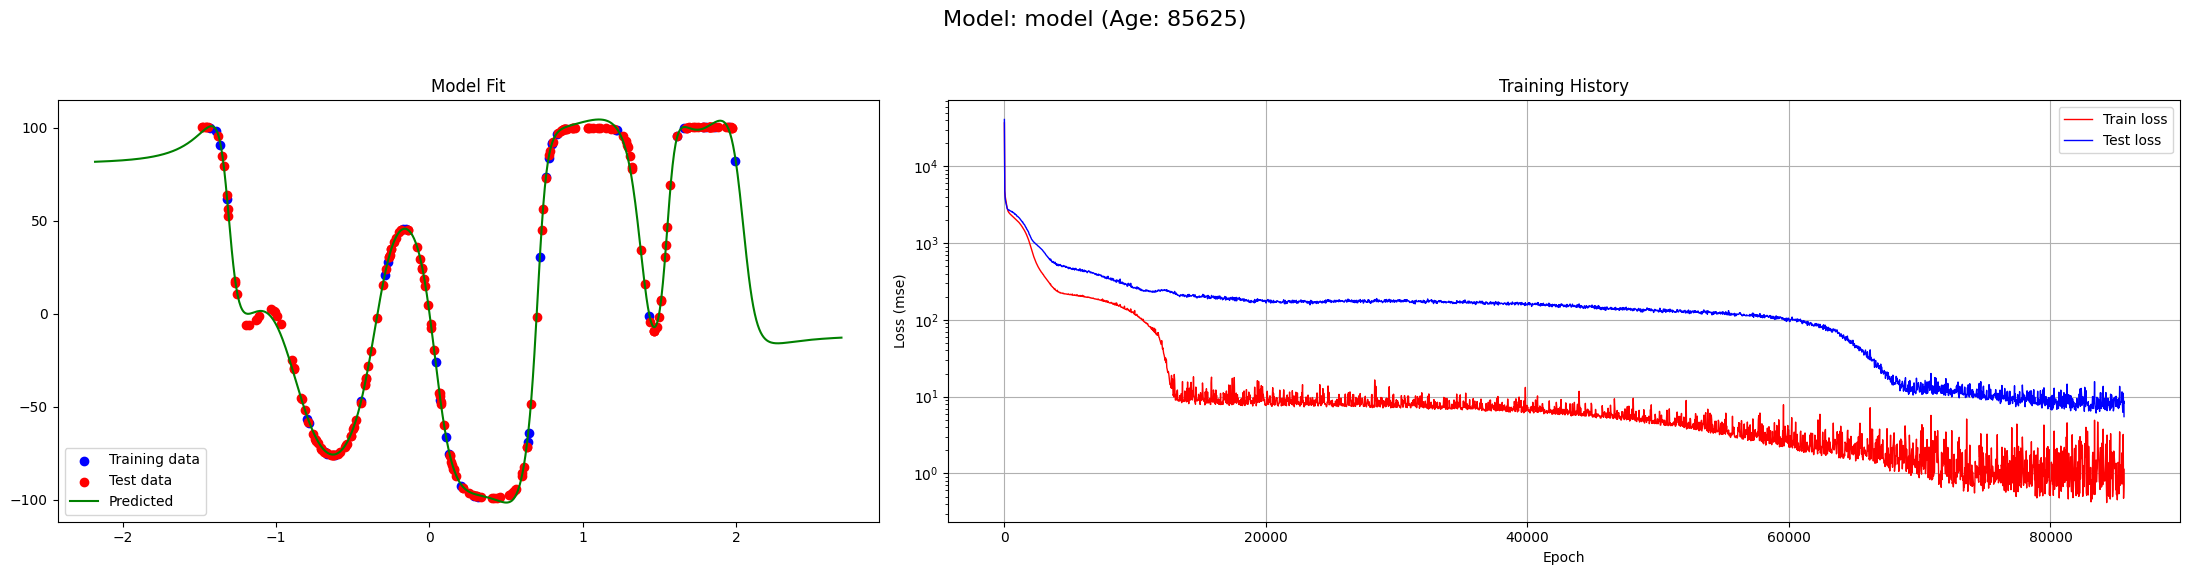
\includegraphics[width=\textwidth]{img/nn6/multimodal-sparse.png}
    \caption{Historia uczenia modelu z regularyzacją L2 na zbiorze multimodal-sparse}
\end{figure}

Wyraźnie widać moment, w którym regularyzacja pozwoliła modelowi zminimalizować przeuczanie. Około 70000 epoki MSE na zbiorze testowym zaczyna wyraźnie spadać i zbliża się wyraźnie do wartości MSE na zbiorze treningowym.

\end{document}